\chapter{脊柱和脊髓}

\section{检查方法}

\subsection{脊柱的常规CT扫描}

\subsubsection{平扫}

①常规仰卧位,颈段可采用头屈曲位,腰段采取双膝屈曲位;②检查颈和胸椎间盘用1~3mm层厚,腰椎间盘用3~5mm层厚,对其他病变一般用5mm层厚;③适当应用软组织窗和骨窗观察。

\subsubsection{增强扫描}

一般平扫即可;必要时可做静脉增强扫描,一般应用60%泛影葡胺80~100ml,团注扫描。

\subsubsection{螺旋扫描}

可行三维重建,以及矢状、斜面、曲面等多平面重建(MPR)。骨性椎管CTVE可用于观察椎体增生、脊椎滑脱和骨折等对骨性椎管的影响。

\subsection{脊髓造影CT(CTM)}

CTM应按下列步骤进行:①检查前2小时禁食。②造影前30分钟静脉注射50%葡萄糖40ml和维生素B\textsubscript{6}
50mg,肌注安定10mg。③腰穿时患者取侧卧位,常规消毒铺巾,取7号腰穿针从L\textsubscript{3}
、L\textsubscript{4}
椎间隙进入硬脊膜后,取脑脊液5ml送常规及生物化学检查,然后缓慢注入30%伊索显或欧乃派克等非离子性造影剂15~20ml(亦有人主张5~10ml以免过多造影剂影响图像质量)。④腰穿注药后应嘱患者翻身,行胸段或颈段CTM者胸膝卧位后CT扫描;亦可嘱患者取仰卧位将臀部垫高30cm,15分钟后行CT扫描。⑤CTM检查后患者必须去枕卧床12小时,床头抬高10°~15°,术后禁食4小时。

\section{正常解剖和CT表现}

脊柱有33块椎骨组成,颈椎7个、胸椎12个、腰椎5个、骶椎5个及尾椎4个(亦可为3~5个)。由于骶、尾段各椎骨相互融合成一骶骨和尾骨,故脊柱亦可说有26块脊椎骨组成。在第1、第2颈椎之间因寰椎无椎体而无椎间盘,骶骨及尾骨因融合亦无椎间盘。其他各相邻椎骨的椎体之间均有椎间盘。

\subsection{椎骨}

\subsubsection{椎骨的解剖结构}

椎骨一般由椎体和椎弓两部分组成,两者合而形成椎孔。①椎体:位于前部,为椎骨最大和负重的部分,由颈椎向下负重逐渐增加而体积逐渐增大,至第4、第5腰椎和第1骶椎体积最大,再向下又逐渐变小。②椎弓:由椎弓根、椎板、棘突、横突及关节突组成。相邻椎骨的关节突之间组成滑膜关节。

除上两个颈椎及骶尾骨以外,相邻椎骨的椎体之间由椎间盘构成关节。椎骨不含骨髓腔,主要由松质骨构成,外围是一薄层密质骨,椎体部的密质骨很薄,而椎体附件处的密质骨则较厚。

\subsubsection{各段椎骨的解剖特点}

1.颈椎:椎体较小,呈椭圆形或方盒状,C\textsubscript{3}
至C\textsubscript{7}
体积逐渐增大,上缘两侧上翘形成钩突,相应椎间盘及上一个椎体的下缘内缩,形成钩椎关节,亦称为Luscka关节。该关节部分填充滑膜,部分填充结缔组织,无关节囊。其椎体后缘平坦,横突根部有横突孔,为椎动脉、椎静脉及神经之通道,一般横突孔横径大于前后径,横径(5.5±1.0)mm,前后径(4.8±0.9)mm。其棘突短而呈分叉状。第1颈椎即寰椎呈环状,无椎体、棘突和关节突,由前弓、后弓和两个侧块组成。第2颈椎即枢椎,其椎体上面有一齿突,齿突的前后面均有关节面存在,分别与寰椎的齿凹和寰椎横韧带相接。第7颈椎形态与上胸椎相似,棘突长而水平,无分叉。

2.胸椎:椎体后部有一对肋凹与肋骨头相关节,由于在个体发生过程中第2~9肋头上移,与上一节胸椎椎体相关节,故第2~8胸椎椎体两侧各有一个上肋凹和一个下肋凹。胸椎的棘突细长,指向后下方,彼此迭叠。胸椎的关节突关节面略呈垂直的冠状位。

3.腰椎:在所有椎骨中体积最大,椎弓根短而粗,向后略偏外平伸。关节突的关节面略呈矢状位,向下逐渐变为斜位。其棘突呈长方形,向后呈水平方向走行。

\subsection{椎间盘}

椎间盘主要由纤维环、髓核、透明软骨终板组成。①纤维环:位于四周,由坚硬的致密纤维软骨构成,椎间盘的最外层为胶原纤维(即所谓Sharpey纤维)所构成,可与前、后纵韧带相混。纤维环主要为分层排列成同心圆的纤维软骨,是椎间盘维持负重的最主要组织。②髓核:位于中央,一般位于椎间盘中部略偏后。主要由黏液状物质所组成,10岁前含水达85%~88%,10岁以后其水分所占比例可随着年龄的增加而逐渐减少,并逐渐为纤维软骨样物质所取代。③软骨终板:即椎体的上下软骨面,形成了髓核的上下界,与相邻椎体分开。

颈、腰部椎间盘较厚,胸部则较薄。颈椎间盘前部较厚,其前缘的高度约为后缘的2~3倍。胸椎间盘的前后部厚度相近。腰椎间盘前部亦较后部厚,尤以腰5椎间盘最为明显。腰椎间盘较相邻椎体外缘略宽,但不超过1~2mm。

婴幼儿椎间盘血供丰富,主要来源于椎体骨化中心和前后纵韧带血管。约13岁以后其血管迅速减少,成为体内最大的无血管结构,仅纤维环及周围结缔组织有血管和淋巴管分布,其营养来源主要为软骨终板和纤维环的弥散。

\subsection{脊柱的韧带}

脊柱的韧带有前纵韧带、后纵韧带、棘上韧带、棘间韧带、黄韧带、关节囊韧带及横突间韧带等,其中以前、后纵韧带及黄韧带较为重要。①前纵韧带:位于椎体的前面及前外侧面,由枢椎伸展到骶骨前面上部,韧带扁而宽。韧带上端有窄条伸展至枕骨。②后纵韧带:位于椎管内椎体的后面,由枢椎伸展到骶管。上端与由枢椎体至枕骨的覆膜相延续。此韧带在椎间盘后面的部分虽然较宽,但在两侧部分较薄,不及中部厚,故椎间盘向后凸出时,发生于两外侧者多于中线附近者。③黄韧带:为一弹性韧带,它起自上一椎板的下后缘,止于下一椎板的上前缘。中央厚而两侧薄,两侧黄韧带于后部中线处愈合,向两侧伸向关节囊至椎间孔处,可分为内侧的椎板部和外侧的关节囊部。颈部黄韧带较薄,向下逐渐增厚,下腰部可达3~5mm(亦有文献为2~4mm)。一般认为成年后不会增长,其增厚(≥5mm)是脊柱缩短韧带褶曲所致。

\subsection{脊柱的关节}

1.椎体关节:即相邻椎体间由椎间盘构成的关节。

2.滑膜关节:①在颈部椎间盘不伸至椎体周边,而椎间盘两侧相邻的椎体互相接触,形成滑膜关节(但无关节囊)即钩椎关节。②寰枕、寰枢关节:属滑膜关节。③椎弓关节:亦称为椎间小关节、关节突关节。由上位脊椎的下关节突与下位脊椎的上关节突所构成。颈椎小关节间隙方向与水平面平均成45°角,下颈椎关节面趋于水平;胸段椎间小关节间隙方向与水平面成60°角,与冠状面平行。腰椎之小关节间隙方向与水平面成90°角,关节间隙由上至下由矢状位渐趋于冠状位。

此外,还有腰骶关节、骶尾关节、骶髂关节、肋椎关节等共同参与脊柱的关节构成。

\subsection{椎管}

椎管前壁为椎体、椎间盘及后纵韧带,后壁为椎板及其间的黄韧带,侧壁为椎弓根及其间的椎间孔,后外侧为椎间小关节。椎管在颈部及腰部较为膨大,以容纳脊髓的颈膨大和腰膨大部。

各段椎管形态不一。①颈段椎管:近似三角形,矢径短、横径长。一般C\textsubscript{1}
的矢径最大,由上而下矢径逐渐减小,C\textsubscript{5}
、C\textsubscript{6}
最窄。颈椎管的平均矢状径约为15mm,C\textsubscript{1}
、C\textsubscript{2} 不应<15mm,C\textsubscript{3~7}
不应<12mm。②胸段椎管:大致呈圆形,其矢径除T\textsubscript{12}
稍大外,其余大致14~15mm;横径除T\textsubscript{1~3}
及T\textsubscript{11} 、T\textsubscript{12}
稍大外,其余大致与矢径相同;胸椎之孔径在整个椎管中最小。③腰段椎管:在L\textsubscript{1}
、L\textsubscript{2} 多呈卵圆形,L\textsubscript{3} 、L\textsubscript{4}
约三角形,L\textsubscript{5}
多呈三叶形。腰椎椎管矢径平均15~25mm,应大于12mm;横径为20~30mm。

侧隐窝:侧椎管是指骨性椎管的外侧部,常分为3个区,即入口区、中间区与出口区。侧隐窝为侧椎管入口区,其前界为椎体后外缘与相邻的椎间盘,后面为上关节突前面与椎板和椎弓根连接处,外面为椎弓根的内面,内侧为硬膜。由于L\textsubscript{5}
椎孔呈三叶形,其侧隐窝明显、矢径小,所以该节段易引起侧隐窝狭窄。其前后径正常>3mm,<2mm则认为狭窄。

椎间孔:由上下相邻的椎弓根、后侧的关节柱与黄韧带、前上部的椎体后外侧与前下部的椎间盘、后纵韧带所组成,呈倒置的泪滴状,上宽下窄。腰部一半以上椎间孔位于椎间盘以上。椎间孔内含神经根袖和脂肪组织。MRI可显示其形态及与椎间盘的关系,但不易辨别神经根袖。腰部神经根袖比颈椎、胸椎高,位于椎间盘的上方。腰部椎间孔高20~23mm,上部(背侧神经节水平)宽8~10mm。

\subsection{脊髓的被膜}

脊髓的表面有3层被膜,由外向内为硬膜、蛛网膜、软膜。

1.硬脊膜:由致密纤维结缔组织构成,呈管状。上方附在枕骨大孔的周缘,与此处的硬脑膜内层相续。其下方为一盲端,约在S\textsubscript{1~2}
、S\textsubscript{2}
上缘平面,其下为一向下延伸的纤维索称为硬脊膜终丝,一直下行至尾骨背面,与该处的骨膜相融合。因硬脊膜外面粗糙,与硬脊膜外脂肪中的结缔组织相混,在前正中线上形成小梁与后纵韧带相连。

2.蛛网膜:是贴在硬脊膜内面的一层薄而透明的膜,由松散的胶原纤维、弹力纤维和网状纤维组成。其外面光滑;内面粗糙,发出许多结缔组织小梁与软脊膜相连。其下端亦大约在S\textsubscript{2}
平面形成一盲端。

3.软脊膜:紧贴在脊髓表面,不易与脊髓实质分开,为一层扁平细胞及少量结缔组织构成的薄膜。其内层直接与神经组织相接触,外层含有较大的血管。在脊髓两侧软脊膜增厚形成两条差不多与脊髓等长的齿状韧带,两侧齿状韧带各发出若干齿突,通过蛛网膜下腔、穿过蛛网膜而附着于硬脊膜。

由于蛛网膜与硬脊膜疏松的结合在一起,CT不能区分硬膜与蛛网膜,而统称为“硬膜囊”。

\subsection{脊髓圆锥和脊神经}

脊髓为前后略扁的圆柱形条状结构,上端较大,与延髓相连;下端变尖成为脊髓圆锥。①脊髓与延髓的分界人为的定在锥体束交叉部的最下限,外部可以枕骨大孔平面或C\textsubscript{1}
神经根根丝上缘平面作为分界。②脊髓下端的位置变动在T\textsubscript{12}
到L\textsubscript{3}
之间。正常胎儿在3个月时脊髓与椎管等长,新生儿脊髓终止于L\textsubscript{3}
下缘。中国人脊髓末端在成人最常见的是L\textsubscript{1}
中下份,儿童则多位于L\textsubscript{2}
平面。脊髓圆锥与硬膜囊二者之间位置不相关。脊髓圆锥向下延续为终丝(终丝内无脊髓组织,仅由软脊膜和室管膜构成,与硬脊膜终丝非同一概念)。

脊髓横断面的横径都大于前后径。脊髓表面有前正中裂、后正中沟。脊髓由灰质和白质构成,新鲜横切面上可见中央部的H形灰暗色灰质,外周为颜色发白的白质。灰质中央又一小孔称中央管,贯穿脊髓全长,向上通第四脑室,向下达终丝的始部,并在脊髓圆锥内呈梭形扩大形成终室。终室一般长15~20mm,宽1~4mm,平扫不易显示。

脊神经有31对,即颈8对、胸12对、腰5对、骶5对和尾1对。第1~7颈神经在相应椎骨的上缘穿出,第8神经在第7颈椎下缘穿出,胸、腰、骶、尾神经都在相应椎骨的下缘穿出。

\subsection{椎管内间隙}

椎管内间隙由以下间隙所构成:

1.硬膜外间隙:即硬脊膜外面与骨性椎管之间的腔隙。其中充以疏松结缔组织、脂肪、淋巴管、椎管内静脉丛及小动脉。硬膜外间隙内的椎内静脉丛,由在椎体后面走行的两条纵行的前内静脉丛及在硬脊膜后外形成的两条后内静脉丛组成,均贯穿椎管全长,并与椎管外静脉丛之间有丰富的吻合;来自节段动脉的脊柱动脉,经椎间孔入椎管,并分支在硬膜外间隙形成纵行动脉,与静脉丛伴行。

2.硬膜下间隙:硬脊膜内面光滑,与其内层的蛛网膜紧密相贴,其间存在的潜在间隙称为硬膜下间隙或硬膜下腔,其内仅有少量具有润滑作用的浆液。

3.蛛网膜下腔:即蛛网膜与软脊膜之间的腔隙,其间充满脑脊液。在胸部该间隙特别窄;在腰部较宽大;在脊髓末端至S\textsubscript{2}
平面处特别宽大,称为终池或腰池,其内含有马尾神经。一般颈段蛛网膜下腔从枕大孔到C\textsubscript{2}
逐渐变小;从C\textsubscript{3} ~C\textsubscript{7}
前后径大致相同,平均约12mm;胸段前后径约12~13mm,T\textsubscript{9}
~T\textsubscript{12} 节段比上部节段略大。

在脊髓软膜表面可见环绕脊髓并与前后动脉相联系的分支,称为动脉冠。自椎动脉分出的1条脊髓前动脉和两条脊髓后动脉,分别下行于前正中裂和两侧脊神经后根基部。脊髓的静脉与动脉相似,但脊髓的前后静脉皆趋向为一单干,并与延髓静脉相交通,且在不同平面向外汇入根静脉。

\subsection{骨性脊柱的CT表现}

①椎体呈圆柱形结构,主要由松质骨构成,表面有薄层皮质骨。②在椎体中部前面和后面都有椎体静脉通过的小孔,CT上表现为皮质不连续,并与松质内呈Y形的低密度线条影相连,不要误为骨折。③椎体后方静脉孔常有垂直之骨质间隔,在横断面上表现为一游离的致密骨,有时还略向外凸,勿误为骨质增生或后纵韧带骨化。④由于椎体内骨髓成分随年龄的增大红骨髓逐渐减少,代之以脂肪性的黄骨髓(20岁时红骨髓占80%,70岁时占40%~50%),故CT上青少年时椎体表现为磨玻璃样基质,其中分布有稍高密度点条状骨小梁。随年龄增加基质高密度逐渐减低。⑤骨质疏松时为基质中许多斑点状的小低密度灶。⑥各段椎管形态不一。

\subsection{椎间盘的CT表现}

1.密度:椎间盘呈软组织密度,CT值约为80~120Hu(或50~110Hu),不能区分髓核和纤维环。通常椎间盘周缘密度要比中央高,主要因周缘含有大量纤维组织及与邻近椎体终板相连的部分容积效应所致。

2.形态:①颈椎间盘:除了在后外侧椎间盘受到钩突的限制,椎间盘的边缘与相邻的椎体边缘一致。②胸段椎间盘:与相邻胸椎体边缘一致。③腰段椎间盘:L\textsubscript{1/2}
至L\textsubscript{3/4}
椎间盘形态大致相似,呈肾形,其后缘略凹,凹陷部与后纵韧带的走行一致;L\textsubscript{4/5}
椎间盘后缘略平直;L\textsubscript{5} /S\textsubscript{1}
椎间盘的后缘可轻微后膨,但硬膜囊无受压表现(图\ref{fig23-1})。

\begin{figure}[!htbp]
 \centering
 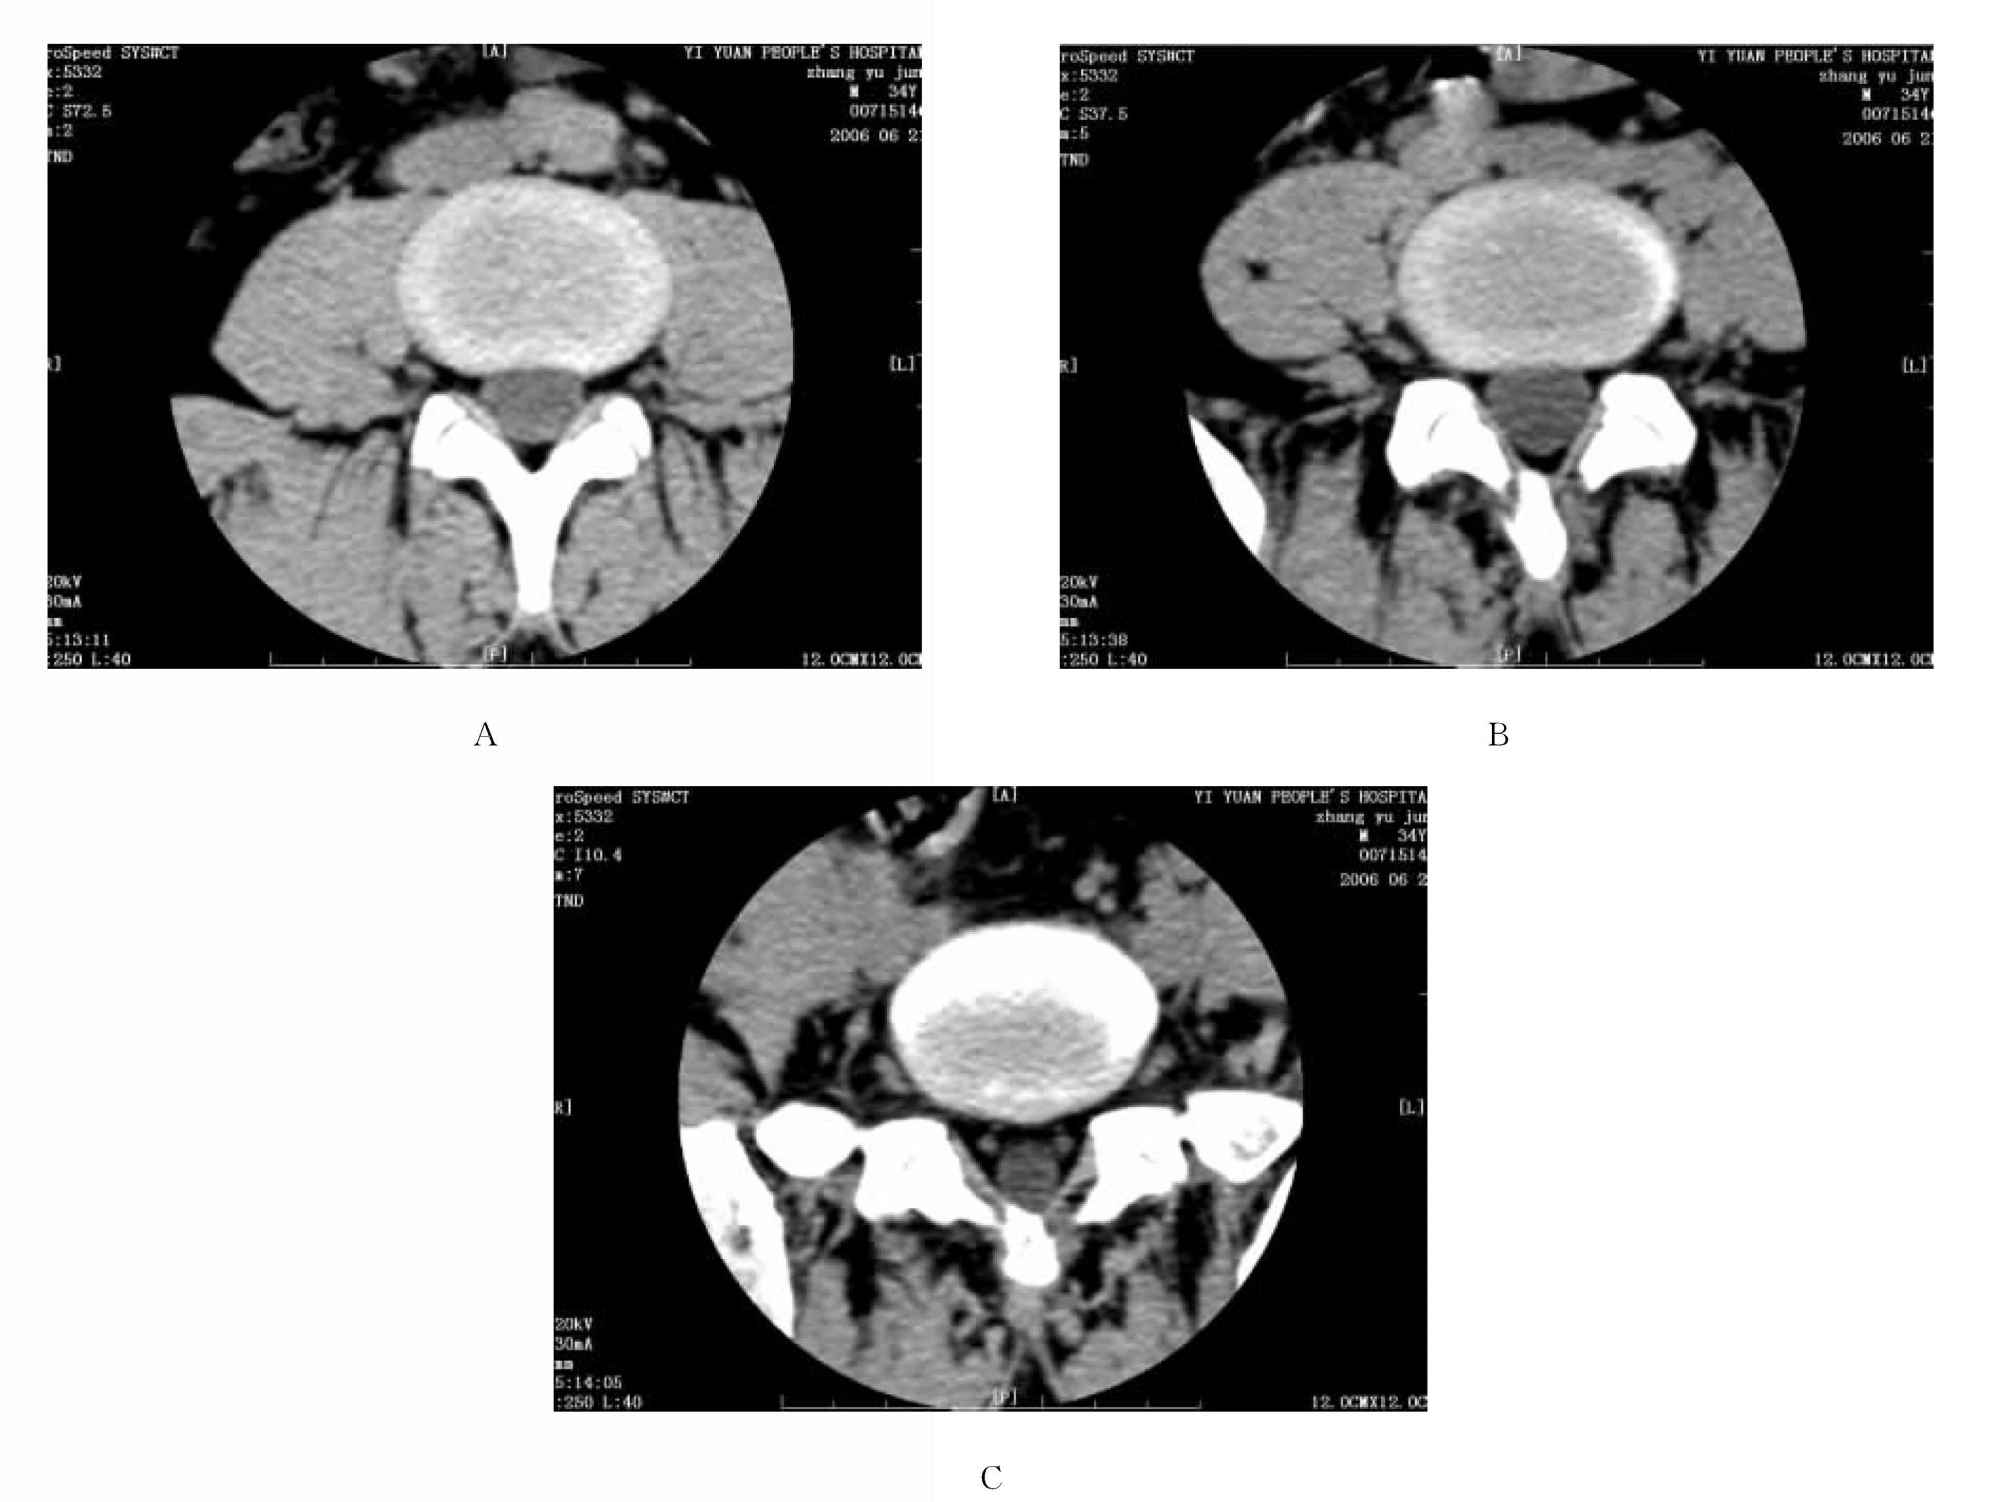
\includegraphics[width=.7\textwidth,height=\textheight,keepaspectratio]{./images/Image00464.jpg}
 \captionsetup{justification=centering}
 \caption{正常腰椎间盘}
 \label{fig23-1}
  \end{figure} 

A.L\textsubscript{3/4} 椎间盘;B.L\textsubscript{4/5}
椎间盘;C.L\textsubscript{5} /S\textsubscript{1} 椎间盘

此外,应注意在CT扫描时,由于扫描线不能与相应间隙平行,(尤其是L\textsubscript{5}
/S\textsubscript{1}
间盘)在椎体上或下缘层面上,椎体的前方或后方出现部分椎间盘影缘,称之为倾斜伪影,勿误认为椎间盘膨隆或疝。

\subsection{椎间小关节及韧带的CT表现}

1.椎间小关节:①关节面彼此平行,关节间隙宽约2~4mm;②软骨下骨质密度均匀,皮质骨与松质骨界限分明;③关节面边缘光滑。

2.韧带:①前、后纵韧带:胸段较颈段和腰段略厚。但前、后纵韧带除了出现钙化,一般CT无法与椎体和椎间盘结构相区分。②黄韧带:密度介于鞘膜囊和椎间盘之间,与肌肉CT值相近。其厚度在颈椎<1.5mm;胸椎<2mm;在腰椎约3~5mm,>5mm可诊为增厚。③其余韧带在适当的层面可予显示。

\subsection{硬膜外间隙的CT表现}

硬膜外间隙含有神经、血管、脂肪和结缔组织。椎内静脉丛密布于椎管的骨膜和硬脊膜之间。平扫时,这些椎内静脉丛不能与其周围组织相区别,但CT增强扫描或直接在椎静脉内注射造影剂后做CT扫描,可使硬膜外间隙明显强化。

硬膜外间隙的脂肪:①在颈段相当少,颈胸交界段有时可以显示其硬膜外脂肪;②在胸段较明显,主要分布于两侧椎弓与硬膜间,而硬膜前方几乎没有;③在腰段脂肪组织较多,常见于硬膜囊前方、硬膜囊与两侧椎板黄韧带之间及两侧隐窝内。

\subsection{马尾神经及脊神经的横断面CT表现}

脊髓位于椎管的中央,由于脊髓周围蛛网膜下腔内脑脊液的衬托,可在CT上显示脊髓的形态结构。静脉增强扫描由于脊髓的强化,可使其形态显示的更清楚一些。CTM更加有利于其显示。

1.颈段:①脊髓在横断面上呈椭圆形,位于蛛网膜下腔的中央,前缘稍平,可见前正中裂形成的浅凹陷,后缘略圆隆,后正中沟常不能显示。②解剖上从C\textsubscript{3}
~T\textsubscript{2}
之间脊髓有一膨大段,但在CT或MR测量上并不明显。③从C\textsubscript{3}
~C\textsubscript{7}
脊髓前后径大致相似,平均约6~8mm,横径约7~12mm,颈膨大横径可达12~15mm。④颈段蛛网膜下腔比较宽大,其前后径与脊髓前后径之比约为2∶1。硬膜囊宽不应<10mm。

2.胸段:①脊髓呈圆形,位于蛛网膜下腔正中稍偏前,亦可见前正中裂,但后正中沟和后外侧沟一般不能显示。②在T\textsubscript{9}
~T\textsubscript{12}
胸椎节段处有个膨大段即腰膨大,然后很快缩小为脊髓圆锥,约至L\textsubscript{1}
或L\textsubscript{2}
平面其下方形成终丝。在CTM上脊髓圆锥或终丝呈硬膜囊中心小圆形充盈缺损。③胸髓的前后径平均在5~7mm,横径7~9mm。

3.马尾:腰、骶、尾神经根(即马尾神经),在硬膜囊中围绕着脊髓圆锥和终丝总称为马尾。CTM表现为位于圆锥与终丝两侧及后方的小点状充盈缺损。常呈V字形或W形排列,其排列和分布较均匀。

4.脊神经:神经根鞘走行于硬膜外脂肪和椎间孔中,内含脊神经根。CT平扫显示神经根鞘为直径约1~3cm的圆形影,位于硬膜囊前外方侧隐窝内,呈脑脊液密度。CTM在神经根穿出层面,可清楚显示脊神经的前根和后根。前根较细、后根较粗,呈条状低密度充盈缺损,并可见在椎间孔处相连合为脊神经。

\section{脊柱与脊髓的先天性异常}

\subsection{概述}

\subsubsection{开放型神经管闭合不全}

本病是指神经组织、骨及其他间充质结构于中线不能完全闭合。其特点为神经组织经脊椎骨的缺陷突出,暴露于外,多数临床即可诊断。主要包括脊髓膨出和脊髓脊膜膨出。

\subsubsection{隐性神经管闭合不全}

本病是指表面有皮肤覆盖的、无暴露的神经组织及囊状结构的神经管闭合不全和相关中胚层结构异常。包括脊膜膨出、背侧皮窦、脊柱脂肪瘤,以及少见的尾侧细胞团管腔化与退变性分化异常(包括脊髓栓系、终丝紧张综合征及尾侧脊柱异常等)、脊髓纵裂等。

\subsubsection{尾侧脊柱异常}

尾侧脊柱异常是尾侧细胞团管腔化与退变性分化异常的一部分。尾侧脊柱异常是指胚胎尾侧发育障碍而形成的异常。尾侧脊柱异常包括:①尾侧退化综合征:除有脊柱、脊髓与脊膜的尾侧部分异常外,还合并有肛门闭锁、生殖器官异常、肾脏发育不良或不发育等。畸形的严重程度可有很大差异,从单发、无症状的尾椎缺如,到腰骶发育不良,极严重的病例可仅发育至T\textsubscript{11}
或T\textsubscript{12}
。②尾端脊髓囊状膨出。③骶前脊膜膨出。④隐性骶内脊膜膨出。⑤骶尾部畸胎瘤(见二十一章第七节)。

\subsubsection{脊索分裂综合征}

脊索分裂综合征为一组先天性异常。胚胎期内由于脊索分裂,局部神经管亦被诱导形成完全或不完全的分裂状态,并且常伴有与皮肤外胚层或原肠的永久性粘连。最严重的畸形为背侧肠瘘,但罕见。其他畸形如脊髓纵裂、肠源性囊肿等相对常见。

\subsection{脊髓膨出和脊髓脊膜膨出}

\subsubsection{脊髓膨出}

为胚胎第1~2周时神经管闭合不全,神经外胚层与皮肤外胚层局部未能分离。多发生于腰骶部,中线神经基板裸露,与两侧皮肤平齐,软膜、蛛网膜下腔及蛛网膜仅见于神经基板腹侧。硬膜亦于背侧缺损。

\subsubsection{脊髓脊膜膨出}

来源于胚胎时期神经管闭合障碍,与脊髓膨出不同的是,同时有脊膜膨出、蛛网膜下腔增宽。病变常见于腰骶部,颈胸部罕见,最常见的相关畸形为ChiariⅡ型畸形(100%),其次为椎管内脊髓脂肪瘤(约3/4),偶见皮样囊肿或上皮样囊肿。中枢神经系统积水常见,如脑积水(80%)、脊髓中央管积水(30%~75%)及无室管膜内衬的脊髓空洞(20%),还可并发胼胝体发育不良、脊髓纵裂等,亦可并发脊柱侧弯(20%)以及脊柱后凸、前凸、髋畸形。本病女婴多见,多无家族史。

影像检查可显示膨出的脊髓或脊髓脊膜、神经根等,但检查的主要目的是观察畸形范围及有否其他相关畸形。

\subsection{脊膜膨出}

\textbf{【病理】}
主要为经脊柱骨缺损向外疝出的脑脊膜囊,内含蛛网膜与脑脊液,不含神经组织,囊表面覆盖正常皮肤。病变大小不一。80%发生于腰骶部。

\textbf{【临床表现】}
本病罕见,约为新生儿的万分之一,男女患病率相近,无神经系统症状和体征,故较小膨出常在成年后诊断或偶然发现。表现为皮下柔软的肿块。

\textbf{【CT表现】}
可见病变处脊柱裂,缺损处椎板变薄外翻,硬膜囊经缺损处疝出,可达皮下。疝囊边缘光滑锐利,呈水样均匀密度。CTM可见疝出的硬膜囊造影剂充盈;囊内无神经根,与脊髓脊膜膨出不同。

\subsection{背侧皮窦}

本病罕见,发生于胚胎原始神经管形成期。

\textbf{【病理】}
神经外胚层与皮肤外胚层局部分离失败,形成粘连,间充质随后填充于原始神经管与皮肤外胚层之间。脊髓上移过程中,粘连牵拉、延长,形成以内衬上皮、连接脊髓与皮肤的条索状窦腔。窦腔自皮肤向内延伸,距离可长可短,短者仅终止于皮下,长者则经中缝或分离的椎板与硬膜相连。约1/3~2/3病例的皮窦进入椎管,皮窦进入椎管后向上延伸达数节段,至病变皮肤相应的脊髓阶段。约50%以上发生于腰骶部,其次为枕部和胸椎。约50%以上的病例合并有皮样或上皮样囊肿;皮样、上皮样囊肿的患者合并背侧皮窦者约20%~30%。

\textbf{【临床表现】}
多见于儿童,无性别差异。多无明显症状,继发感染时可出现相应症状,合并皮样或上皮样囊肿可触及肿块。病变处皮肤可见小凹或小孔,周围常有色素沉着、毛痣或毛细血管瘤。

\textbf{【CT及CTM】}
可见病变处皮下脂肪内带状软组织密度结构横过,经开放的椎弓板进入椎管,深度不一,近端止于硬膜,也可进入硬膜与圆锥或终丝相连。合并有椎管内皮样或上皮样囊肿时,带状窦的近端常止于囊肿。

\subsection{脊柱脂肪瘤}

本病为椎管或椎管内外脂肪纤维组织肿块,与脊髓或脊膜相连,为隐性骶裂最常见的并发异常。依据肿瘤发生的部位及合并的其他异常将其分为3类。

1.脂肪脊髓脊膜膨出

约为脊柱脂肪瘤的84%,占隐性椎管闭合不全的50%以上;表面皮肤完好的骶部肿物约20%为脂肪脊髓脊膜膨出。病变由脂肪瘤加上膨出的肌肉纤维囊构成,脂肪常经疝囊的缺损进入囊内。

\textbf{【临床表现】}
多见于6个月前婴儿,女性居多。由于脊髓栓系低位,常有神经性膀胱与鞍区感觉异常。可见腰骶部较大皮下肿物,局部表面皮肤完整,可有色素沉着。

\textbf{【CT与CTM】}
①可见腰骶皮下大的脂肪密度占位,常经腰骶部椎弓板裂进入椎管。②脊髓低位,圆锥(神经板)与背侧硬膜囊不分离,结构不清。③神经根向前穿过宽大的蛛网膜下腔进入神经根袖。④25%的患者合并脊髓空洞,也可合并ChiariⅠ型畸形,但不合并ChiariⅡ型畸形。

2.终丝纤维脂肪瘤

终丝纤维脂肪瘤来源于尾侧细胞团退缩性异常,可分为终丝大纤维脂肪瘤与小纤维脂肪瘤。

\textbf{【临床表现】} 临床无症状,多偶然发现。

\textbf{【CT及CTM】}
①大纤维脂肪瘤多附着于终丝背侧,终丝局部增粗,脂肪密度;②小纤维脂肪瘤常位于终丝内(图\ref{fig23-2})。

\begin{figure}[!htbp]
 \centering
 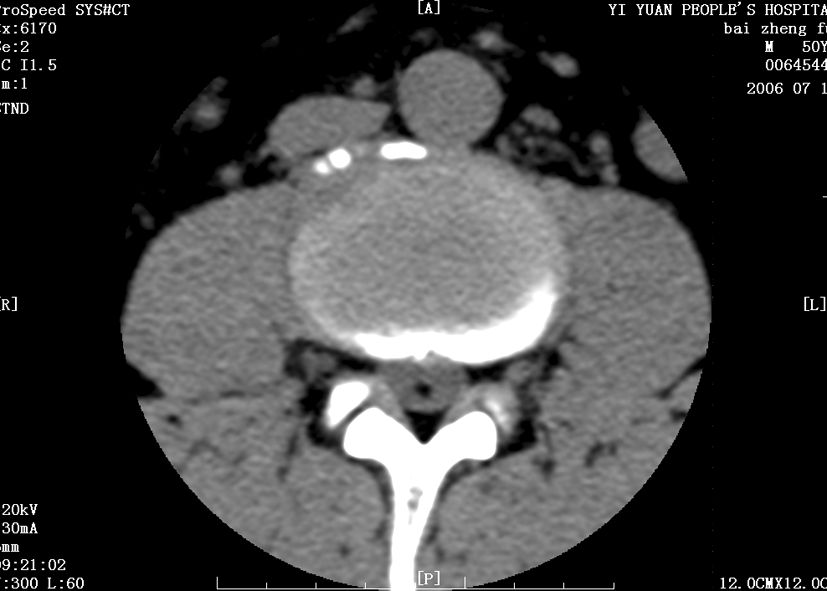
\includegraphics[width=.7\textwidth,height=\textheight,keepaspectratio]{./images/Image00465.jpg}
 \captionsetup{justification=centering}
 \caption{终丝纤维脂肪瘤\\{\small 终丝区有近圆形脂肪密度灶,边缘清晰}}
 \label{fig23-2}
  \end{figure} 

3.硬膜内脂肪瘤

亦称为软膜下脂肪瘤,少见。多不合并其他脊柱脊髓畸形,常发生于颈、胸段脊髓背侧。

\textbf{【临床表现】}
发病高峰年龄为5岁以下(24%);20~40岁(55%);50~60岁(16%)。男女发病率无差异。临床上可有进行性下肢无力与步态异常。

\textbf{【CT表现】}
平扫可见脊髓背侧局限性脂肪密度占位,常呈分叶状。小脂肪瘤CT不及MR敏感。

\subsection{特发性硬膜外椎管内脂肪增多症}

本病罕见,是指非柯兴病(包括原发或继发性)性硬膜外脂肪增多。发生于胸段椎管,次为腰骶部。

\textbf{【病因病理】}
本病病因不清,与体胖无肯定关系。表现为椎管内硬膜外脂肪大量沉积,边界不明显,无包膜。

\textbf{【临床表现】}
好发于18~54岁,男性多见。症状缓慢进展,严重时可出现脊髓压迫症状。

\textbf{【CT表现】}
椎管内硬膜外一侧脂肪明显增多,多位于背侧,上下范围可达数节段,呈连续带状或梭形分布,前后径≥8mm;硬膜囊背侧受压变窄。

与范围相对局限、有包膜的脂肪瘤影像学鉴别可有困难。

\subsection{脊髓栓系综合征}

本病为脊髓脊椎等结构的先天性发育异常。脊髓圆锥下移并被栓系在椎管内,同时伴有其他畸形,从而产生一系列神经功能障碍的综合征。

\textbf{【病理】} 脊髓圆锥低于正常,位于L\textsubscript{2}
以下(正常新生儿脊髓终止于L\textsubscript{3}
下缘,成人则在L\textsubscript{1} 、L\textsubscript{2}
椎体之间),终丝增粗变短、部分可伴脂肪变性。还可见脊髓纵裂、椎管内脂肪瘤、脂肪性脊髓脊膜膨出、半椎体及蝴蝶椎、皮毛窦等异常。终丝远端被硬膜周围纤维粘连牵拉。

本病可分为5种类型。①终丝粗大型:最常见,终丝横径>2mm,致圆锥低于L\textsubscript{3}
水平以下;②脂肪瘤型:椎管内脂肪组织包绕脊髓及马尾神经,与硬膜紧密粘连,其中包括腰骶部脂肪瘤型脊膜膨出;③术后粘连型:多为脊膜膨出术后所致;④肿瘤型:包括脊髓内皮样囊肿、神经肠源囊肿、畸胎瘤等包绕脊髓或马尾神经;⑤混合型:为上述两种以上病变同时存在者。

\textbf{【临床表现】}
本病可见于任何年龄,无性别差异。临床症状各异,神经功能障碍表现为大小便失禁、排便排尿困难或伴有下肢功能障碍。25%有脊柱前突或后突。

\textbf{【CT与CTM】} 可见圆锥低位,位于L\textsubscript{3}
以下;终丝增粗,横径>2mm,终丝与圆锥分界不清;有时可见粘连带。螺旋CT的多平面重建(MPR)有利于显示。MPR还可见因圆锥低位致马尾神经短,呈聚拢状进入神经根袖。合并脂肪瘤及其他肿瘤或肿瘤样病变可有相应的表现。

\subsection{尾端脊髓囊状膨出}

本病也称为脊髓空洞性膨出,为脊髓远端囊状扩张。

\textbf{【病理】}
畸形的脊髓低位,中央管积水,扩大的脊髓末端(终室)与脑膜、蛛网膜下腔一起突至皮下。扩大的脊髓末端呈气球样,近皮肤侧较平坦,相应的蛛网膜下腔宽大。还可有脊柱裂或部分骶骨不发育。

\textbf{【临床表现】}
可见骶尾部皮下肿物,局部表面皮肤完整。骶尾部表面皮肤正常的肿块中,约有1%~5%为尾端脊髓囊状膨出。

\textbf{【CT与CTM】}
CTM螺旋扫描MPR像可清楚显示气球样扩大的脊髓末端与蛛网膜下腔突出到皮下,而且可显示相关脊椎骨结构的异常。

\subsection{骶前脊膜膨出}

\textbf{【病理】}
骶前脊膜膨出为经骶尾骨前侧的缺陷或相邻的椎间盘间隙的脊膜疝。表现为盆腔内骶前充满脑脊液的囊,可以是尾侧退化综合征的组成部分,也可与遗传性中胚层发育不良(如神经纤维瘤病Ⅰ型)有关。

\textbf{【CT与CTM】}
骶管扇贝状增宽,边缘光滑;骶前囊状水样密度灶,可单发或多发。CTM可见囊腔与骶管内蛛网膜下腔同时充盈造影剂。

\subsection{隐性骶内脊膜膨出}

\textbf{【病理】}
隐性骶内脊膜膨出主要改变为蛛网膜经硬膜的缺陷疝出,疝囊压迫骶管使骨性骶管扩大。可合并有脂肪瘤、骶部色素沉着、骶尾部皮肤陷凹及神经纤维瘤等。多数疝囊与蛛网膜下腔相通,而无症状;不相通者可有症状。

\textbf{【CT与CTM】}
骶管扇贝状增宽,边缘光滑。CTM交通性疝囊可见含造影剂的蛛网膜下腔(终池)与疝囊间有线状硬膜隔,以MPR显示为佳;非交通性则呈骶管远侧不充盈造影剂的水样密度占位,与其他囊性占位常难以鉴别。

\subsection{脊髓纵裂}

本病是一种少见的先天性脊髓畸形,其病因不明,目前其命名尚不统一。

\textbf{【病理】}
该畸形的形态特征为脊髓或终丝在矢状面上被间隔节段性分开。间隔可以由纤维组织、骨、软骨或上述几种成分组成。典型者病变多局限,分裂的两个半髓多不对称,各具中央管和一侧的前、后角及神经根,粗细均小于正常脊髓,其分裂上下端的脊髓为正常单一脊髓。50%以上合并有脊髓积水;约3/4伴圆锥低位(脊髓栓系),位于L\textsubscript{3}
水平以下;还多伴有背部皮肤异常、脊柱畸形(脊髓)脊膜膨出等。

国外有学者主张分为2种类型。Ⅰ型:分裂的两个半髓分别位于各自独立的硬膜囊中,椎管亦为左右两个,中间为软骨或骨结构分隔。Ⅱ型:两个半髓处于一个共同的硬膜囊内,中间为柔软的纤维性分隔。近期国内有学者主张分为单管型和双管型。

\textbf{【临床表现】}
多见于女性,男女之比约为1∶2~1∶5,症状初发的年龄不一,但求治者儿童多见,成人少见。由于患儿神经发育缺陷,故可能产生一系列神经损害症状,如疼痛、下肢力弱、步态不稳、下肢发育不良、足畸形、神经性膀胱、便秘、二便失禁等。由于本病在胚胎学上影响了3个胚层的发育,故常与其他畸形并存,最常见的是背部表面皮肤异常如多毛症、皮窦、脂肪瘤、血管瘤或皮样囊肿;其次是先天性脊柱侧突(60%~79%)。

\textbf{【CT表现】} 本病主要发生于胸腰段,尤其是L\textsubscript{1}
~L\textsubscript{3} ,其次是胸段,T\textsubscript{5}
以上显著减少,极少见于颈段和骶段;约15%~20%可同时出现胸、腰两处脊髓纵裂。①可清楚显示分裂的两半脊髓所在的椎管与骨性分隔及相关的脊柱异常如半椎体、蝴蝶椎、椎间隙狭窄等,约占85%。60%的患者相邻椎弓板融合,且合并脊柱裂。椎管骨性分隔(骨棘)约占全部病例的1/2,骨棘可为部分性,也可为完全性;可位于正中矢状线上,也可偏于一侧。②CTM可显示共硬膜囊型的矢状纤维分隔及两侧的半髓,椎管增宽,边缘光滑。③MPR可显示相关的畸形,如圆锥低位或栓系、终丝肥厚、中央管积水等。④15%~20%的ChiariⅡ型畸形的患者合并有脊髓纵裂。

\textbf{【鉴别诊断】}
本病应与双干脊髓鉴别(但也有学者主张把两者统称为脊髓分裂畸形),后者两条脊髓均有双侧前后角及双侧神经根,径线也与正常脊髓相近。

\subsection{椎管内肠源性囊肿}

肠源性囊肿罕见。来自胚胎第3周原始肠道形成过程中,前肠与脊索粘连而不能完全分离或遗留的前肠组织残余发育而来。

\textbf{【病理】}
囊肿边界清楚,囊内含清亮液体,囊壁厚。病变多发于胸段椎管内(42%),其次为颈段(32%)、后颅窝及颅颈交界处,腰段罕见。85%~90%位于脊髓或脑干的腹侧中线、髓外硬膜内,偶见位于髓内。

\textbf{【临床表现】}
多见于40岁以下,男性略多见。临床症状轻重不一。常见间断性疼痛及相应脊髓压迫症状,偶见化脓性或化学性脑脊膜炎表现。

\textbf{【CT及CTM】}
可见脊髓腹侧、髓外硬膜囊内长圆形占位,边缘清楚光滑,与脊髓呈锐角相交,密度均匀。增强扫描无强化。

\textbf{【鉴别诊断】}
本病需与髓外硬膜内神经鞘瘤等相鉴别。本病好发于胸段且常伴脊柱发育畸形(如脊柱裂、半椎体、蝴蝶椎等)等有助于诊断和鉴别诊断。

\subsection{脊髓空洞症}

严格讲脊髓积水与脊髓空洞两者并不相同。脊髓积水指脊髓中央管积水,积水周围是室管膜的“壁”;脊髓空洞为脑脊液通过室管膜的裂损聚集于中央管旁,周边无室管膜“壁”。但实际上脊髓空洞与中央管积水常同时存在并多有交通,且临床甚至病理均难以区分。故一般将两者笼统称为脊髓空洞症。所以,脊髓空洞症的概念应为与脊髓中央管有交通或没有交通的、脊髓实质内含有脑脊液的病理性腔隙。

\textbf{【分类】}
脊髓空洞症是一种慢性进行性疾病,但其分类比较混乱。①按空洞是否与蛛网膜下腔或脑室相通分为交通性和非交通性。②按病因分为先天性和后天性,前者多伴有小脑扁桃体联合畸形等先天性发育异常;后者多伴有外伤、肿瘤、髓外占位压迫、蛛网膜炎或变性疾病等许多因素。

\textbf{【病理】}
脊髓内管状空腔形成,周围有胶质组织增生,空洞内液与脑脊液成分相似,洞壁由星形细胞或室管膜细胞构成。当增生的胶质组织在空洞内形成分隔时,空洞呈腊肠样或多房性改变。膨大的脊髓表面可见到扩张的畸形血管。颈髓与上胸髓最易受累,有时可涉及延髓、下胸髓甚至脊髓全长。

\textbf{【临床表现】}
好发于25~40岁,男性略多见。典型者包括感觉特别是痛温觉异常,四肢肌力弱或肌肉萎缩,上肢深反射减弱甚至痉挛性瘫痪。症状严重程度不一,约80%的患者主诉下肢力弱或僵硬,近50%的患者主诉疼痛。不予治疗,则空洞范围可逐渐扩大。

\textbf{【CT表现】}
80%的空洞平扫表现为髓内边界清晰的低密度囊腔,相应脊髓外形多膨大,也可大小正常;病史长者空洞内压力较低,可见脊髓萎缩、外形欠规则。当空洞较小或含蛋白量较高时,平扫可能漏诊。CTM24h延迟扫描(亦有主张8h以上)常可见造影剂充盈空洞而呈高密度。当空洞不直接与蛛网膜下腔相通时,造影剂可通过脊髓血管间隙或第四脑室的交通进入空洞。脊髓肿瘤或其他原因继发者,可出现相应表现;外伤所致者多呈偏心性。

但该病的诊断以MR检查为首选(图\ref{fig23-3})。

\begin{figure}[!htbp]
 \centering
 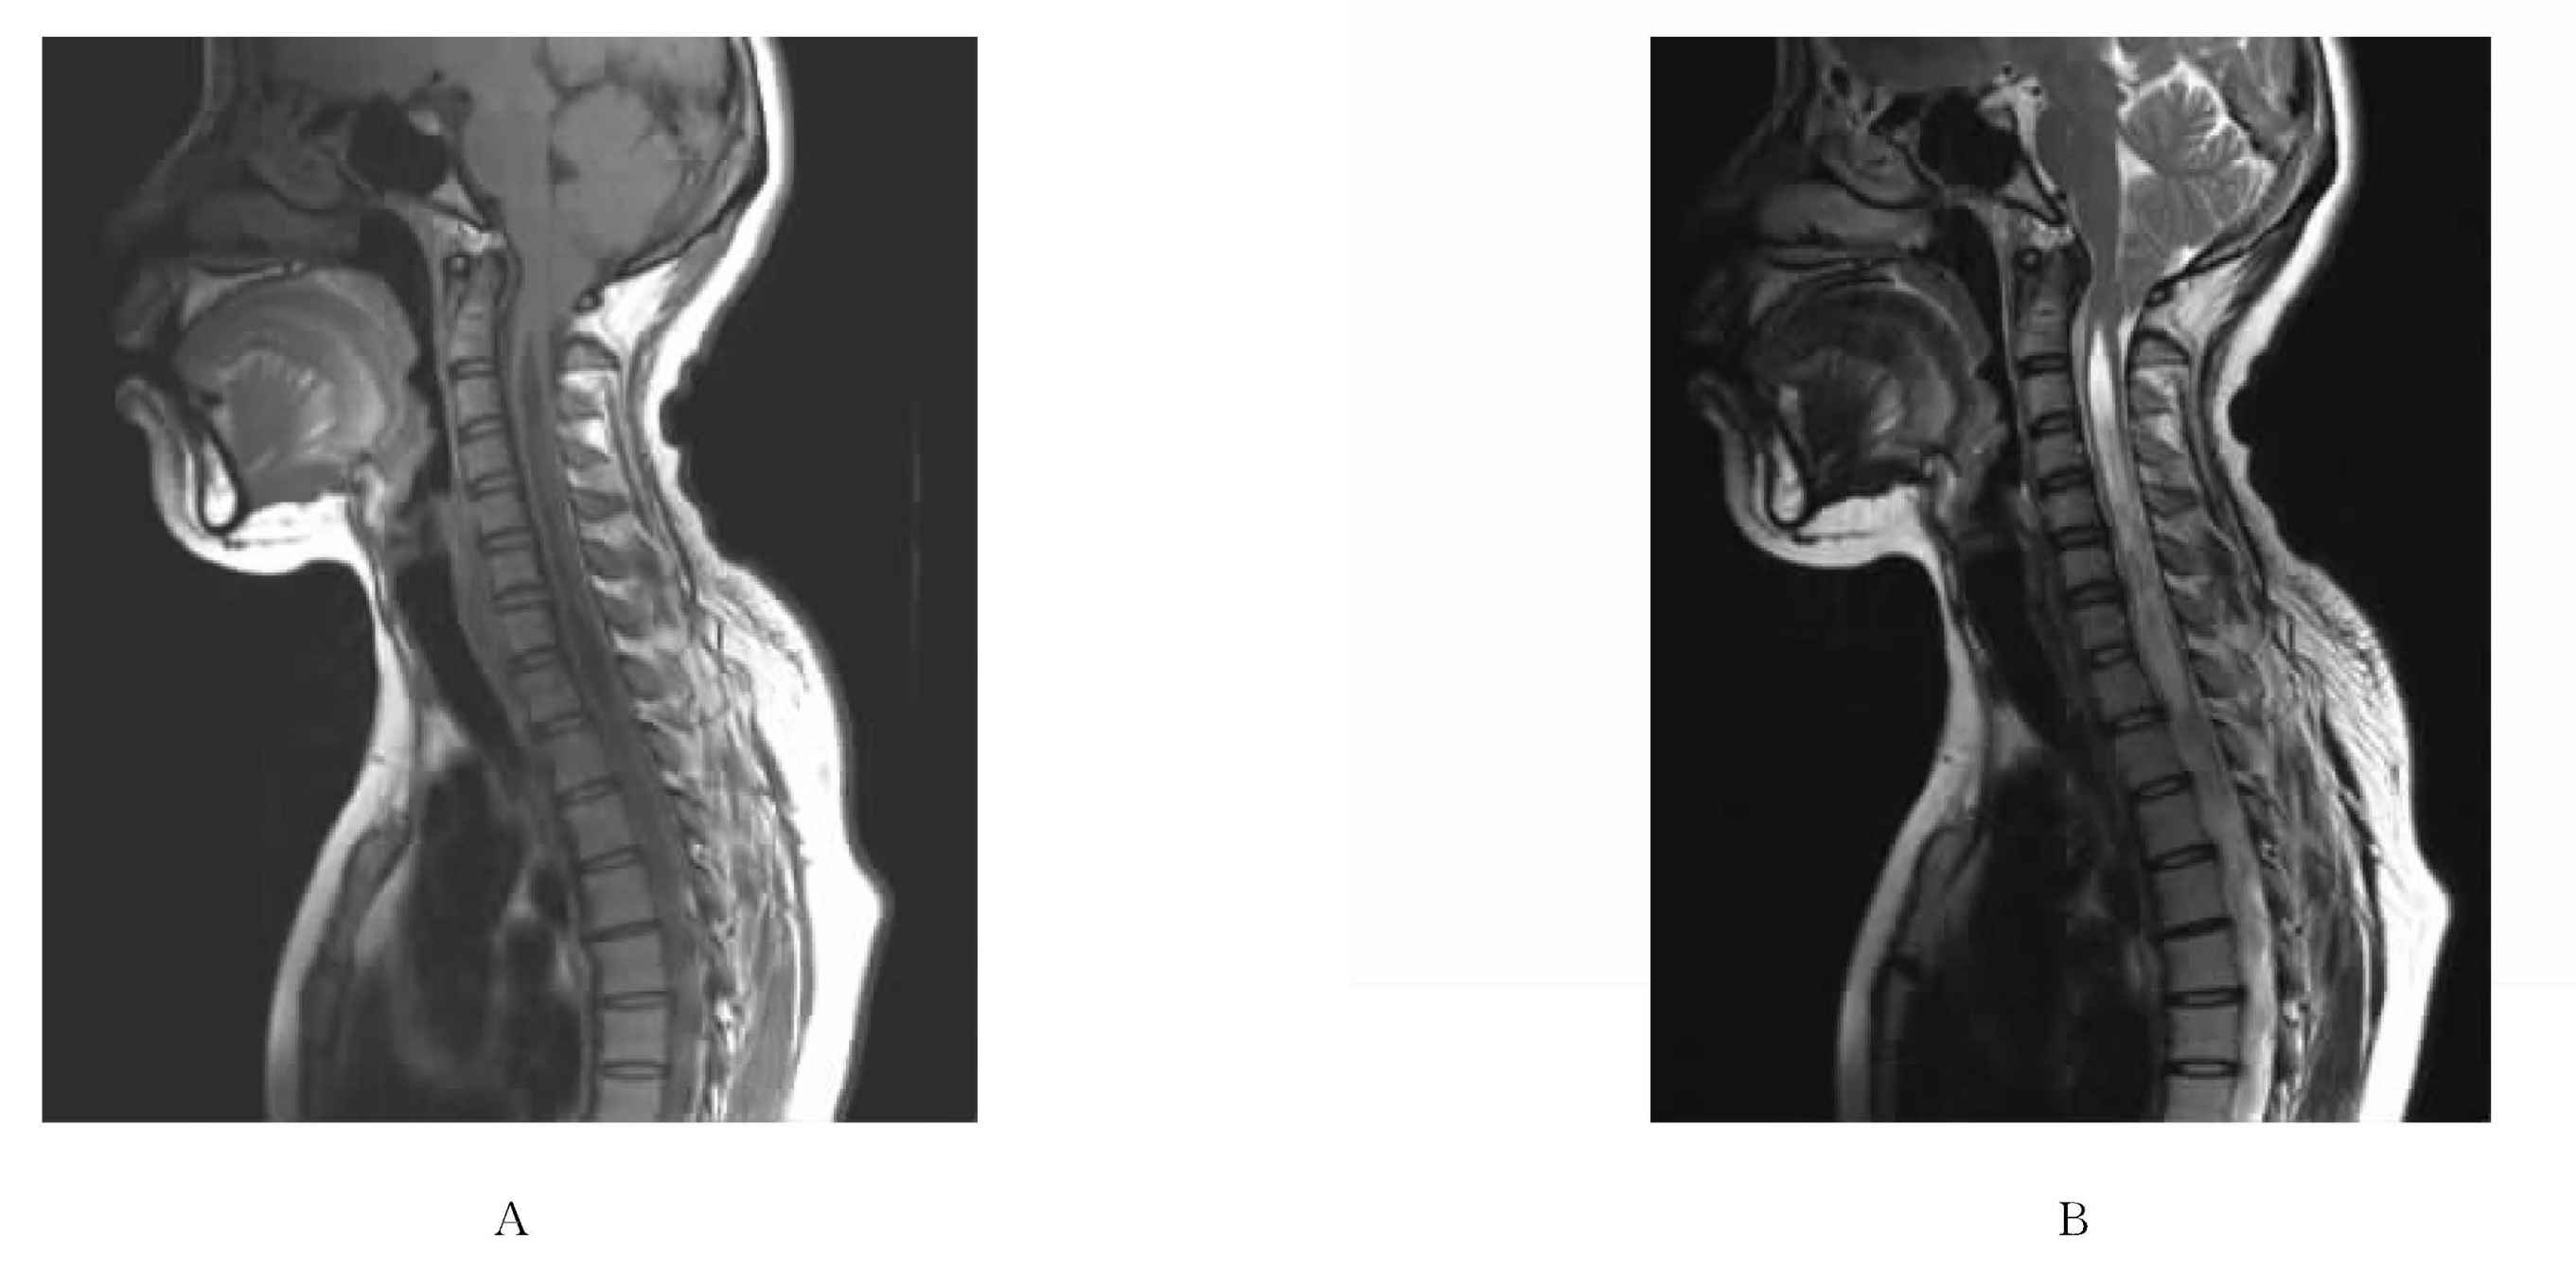
\includegraphics[width=.7\textwidth,height=\textheight,keepaspectratio]{./images/Image00466.jpg}
 \captionsetup{justification=centering}
 \caption{脊髓空洞症}
 \label{fig23-3}
  \end{figure} 

MR表现颈段(涉及部分胸髓)脊髓内可见界限清晰的长T\textsubscript{1}
、长T\textsubscript{2}
信号区;局部脊髓外形膨大。本病例还可见小脑扁桃体下移等ChariⅠ畸形的表现

\subsection{共同神经根鞘}

共同神经根鞘是一种少见的正常变异,偶可并发坐骨神经痛。

\textbf{【病理】} 一般是单侧性的,累及L\textsubscript{5}
和S\textsubscript{1} 神经根,其硬膜囊的发出点介于正常L\textsubscript{5}
与S\textsubscript{1}
神经根发出点之间。两条神经根包含在同一根鞘内,造成两侧根鞘位置、形态、大小的不对称。每条神经根有各自的蛛网膜下腔,内充满脑脊液。

\textbf{【CT表现】}
①共同根鞘的一侧偏大,呈带状,很像位于椎弓根内侧侧旁沟内的软组织肿块,其密度与硬膜囊一致。②CTM可见“软组织肿块”内充盈造影剂,并显示其内的两条神经根,具有特异性。

\textbf{【鉴别诊断】}
应与椎间盘突出和神经源性肿瘤相鉴别。①共同神经根鞘介于L\textsubscript{5}
与S\textsubscript{1}
神经根发出部位之间,密度与硬膜囊一致,与椎间盘关系不密切;而椎间盘突出密度高于硬膜囊,与椎间盘关系密切。②前者呈带状,而不呈结节状或哑铃形,增强扫描无强化,不伴局部椎管骨质改变,可资与神经源性肿瘤相鉴别。此外,CTM对共同神经根鞘的诊断有特异性。

\section{脊柱退行性病变}

\subsection{概述}

\subsubsection{椎间盘退行性变所致纤维环裂隙的病理分型、分度}

椎间盘特别是腰椎间盘的退行性改变为进行性,可贯穿终生。由于椎间盘水分的减少,抵抗能力的下降,而轻度的反复挤压损伤使纤维环出现不同程度的撕裂。CT不能显示,但髓核造影后CT可显示其撕裂的类型、程度与髓核突出的关系。

1.分类:有学者冰冻后切片及显微镜检,将纤维环裂隙分为3种。①同心圆状裂隙:裂隙被液体充填;②放射状裂隙:常伴纤维环断裂,但Sharpey纤维完整;③横行裂隙:纤维环和Sharpey纤维均断裂,有时累及后纵韧带。

2.分度:有学者将放射状撕裂分为3度。Ⅰ度:为不完全撕裂,裂隙不到达椎间盘边缘;Ⅱ度:为完全撕裂,裂隙到达椎间盘边缘;Ⅲ度:撕裂伴有髓核突出,撕裂的深度可贯穿椎间盘的全厚,也可达部分厚度。

总之,纤维环内裂是椎间盘退行性变的象征;而椎间盘膨出和突出亦是椎间盘退行性变的表现。

\subsubsection{椎间盘膨出和突出的病理区别}

1.椎间盘膨出:椎间盘退行性改变,髓核体积缩小,不能充盈纤维环;失水而弹性降低的纤维环承受压力增加、高度下降,纤维环周边膨出,椎间盘直径增大,边缘超出椎体边缘,而髓核位置大致正常。有文献认为20岁以上成人至少有1个腰椎间盘膨出。

2.椎间盘突出:是指椎间盘局限性凸出,超过了椎体边缘,也大多由退行性变所致,偶可为急性外伤性。其突出的部分可以是纤维环,也可以是沿着撕裂纤维环的裂隙向外疝出的髓核,故认为椎间盘突出是单纯髓核突出的观点是错误的。

此外,国外有学者将椎间盘膨出作为椎间盘突出的类型之一。尤其在CT上判断膨出还是突出只能根据椎间盘的外形改变,不能显示纤维环与髓核的病变,诊断“膨出”时不能排除有“突出”的病理改变。总之,膨出与突出无论病理还是CT,尤其CT难以明确区分。

\subsubsection{椎间盘退行性变的CT表现}

1.椎间盘高度降低:程度不一,多数患者不伴有临床症状。腰椎侧位平片及CT矢状重组像可予显示。

2.椎间盘真空变性:据统计20~40岁的人群中35%可出现,60岁以上的人群60%出现。CT可见椎间盘内不规则气体密度区(图\ref{fig23-4})。

\begin{figure}[!htbp]
 \centering
 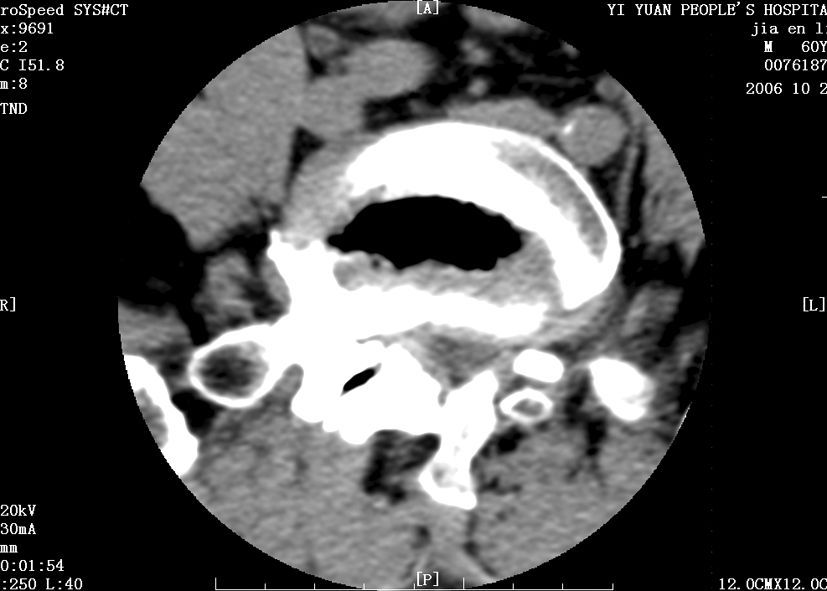
\includegraphics[width=.7\textwidth,height=\textheight,keepaspectratio]{./images/Image00467.jpg}
 \captionsetup{justification=centering}
 \caption{椎间盘积气\\{\small 椎间盘内有近椭圆形低密度气体区,右侧椎间小关节亦有低密度积气表现}}
 \label{fig23-4}
  \end{figure} 

3.Schmorl's(许莫氏)结节:为椎间盘物质在压力的作用下通过终板进入椎体。常见于腰椎,也可见于颈椎。随年龄增长其发生率增加,多不伴临床症状。CT表现与扫描层厚及结节深度有关,薄层扫描可见与终板相邻的椎体内陷入的高密度结节状影,相邻终板层面的相应部位显示近圆形骨缺损,边缘硬化、光滑锐利(图\ref{fig23-5})。

\begin{figure}[!htbp]
 \centering
 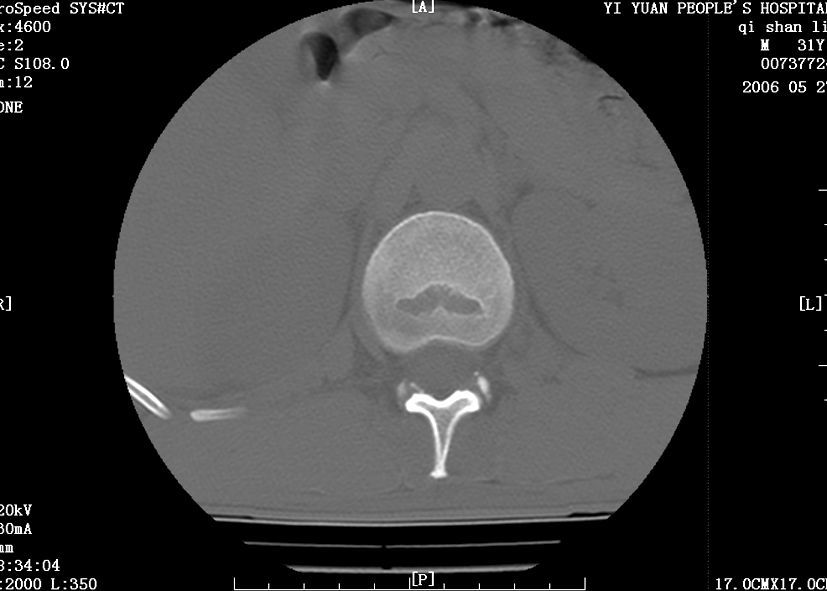
\includegraphics[width=.7\textwidth,height=\textheight,keepaspectratio]{./images/Image00468.jpg}
 \captionsetup{justification=centering}
 \caption{许莫氏结节\\{\small 椎体中后部可见横行低密度区,边缘硬化}}
 \label{fig23-5}
  \end{figure} 

4.椎间盘膨出或(和)突出。

5.常伴有脊柱退行性骨关节病表现。

此外,椎间盘退变可并发脊椎终板骨软骨炎,并引起颈腰背部疼痛。但CT不能显示;MR可见局部信号异常,但无骨质破坏。

\subsubsection{椎间盘突出与膨出的CT区别}

典型局限性突出的椎间盘不难诊断,但隆起的范围多大属于局限。一般认为椎间盘膨出为椎间盘沿椎体向四周均匀性、对称性膨隆。但不均匀、不对称就是突出吗?故对不典型者,“突出”与“膨出”的诊断意见常难以统一。

我们建议隆起的范围如小于椎体周长的1/4(或其圆周的90°)作为局限性隆起,即可诊断为“突出”,而大于周长的1/4者可诊断为“膨出”。尽管如此,有时仍难以区别,而且膨出合并突出者并非少见。

\subsection{椎间盘膨出}

\textbf{【临床表现】}
绝大多数无症状,但当伴有椎管狭窄、神经根受压等改变时可出现腰腿痛。

\textbf{【CT表现】}
椎间盘沿椎体四周较均匀、对称性膨出,即椎间盘平面大于椎体平面,常伴椎间盘高度降低。①轻度时表现为椎间盘后缘正常肾性凹陷消失、圆隆饱满。②重度时弥漫膨出的间盘边缘明显增宽,超出上下椎体边缘,但椎间盘仍对称。③严重时可造成硬膜囊受压狭窄、椎管狭窄等(图\ref{fig23-6})。④可伴有真空变性、钙化以及其他脊柱退行性改变。

\begin{figure}[!htbp]
 \centering
 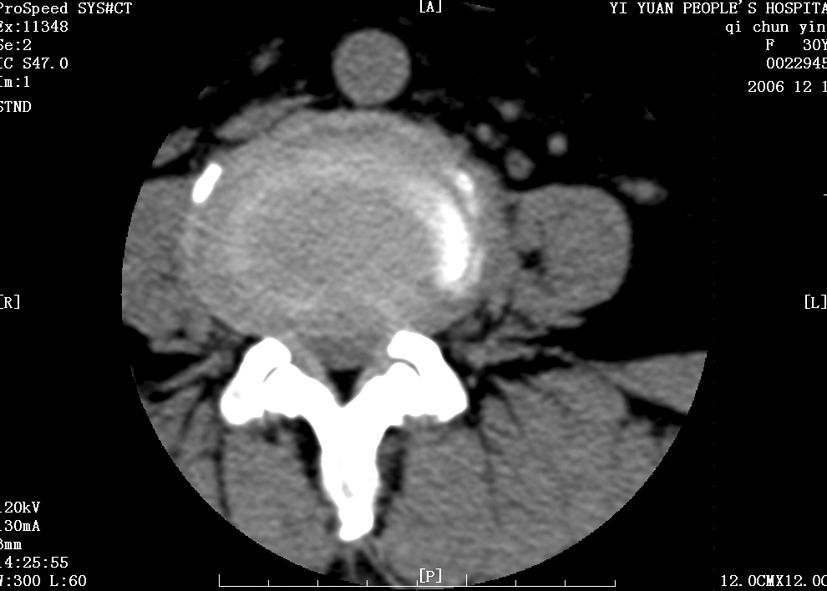
\includegraphics[width=.7\textwidth,height=\textheight,keepaspectratio]{./images/Image00469.jpg}
 \captionsetup{justification=centering}
 \caption{椎间盘膨出\\{\small 椎间盘向四周均匀的膨出}}
 \label{fig23-6}
  \end{figure} 

\subsection{腰椎间盘突出}

\textbf{【病理分型】}

1.依突出程度分型:①椎间盘膨隆:椎间盘沿椎体四周均匀、对称膨出。②椎间盘突出:椎间盘局部轮廓异常,突出之椎间盘位于后纵韧带内,与椎间盘母体呈宽底相连。③椎间盘疝:椎间盘局限性地突入椎管或神经孔,疝出的椎间盘位于后纵韧带之后(提示纤维环和后纵韧带呈完全性断裂),与椎间盘母体呈狭颈相连。④椎间盘游离:椎间盘突出部分断裂、移位,与椎间盘母体完全分离。亦有学者认为以上各型也可再分为轻、中、重度,以便容易被临床医师所接受。

2.依突出方向与受压神经的关系分型:①中央型:亦称正中型,突出部分位于椎管中央,临床以马尾受压为特征。②中央旁型:亦称正中旁型,最多见,突出部分位于椎管中央旁,通常压迫小关节下隐窝内神经根的横行部分。③侧向型:亦称椎间孔型、外侧型,40%位于L\textsubscript{2/3}
和L\textsubscript{3/4}
平面,压迫鞘内神经根或神经节。④过侧向型:亦称椎间孔外型、远外侧型,相对较少,可压迫后神经节。⑤前型:以往很少注意,有作者报道占椎间盘突出的20%。

\textbf{【临床表现】}
可分为急性与慢性腰椎间盘突出。①急性突出:多见于中青年,常有腰部扭伤或其他外伤史。常见腰痛、下肢放射痛,腰背部肌肉保护性痉挛,患侧直腿抬高试验阳性。②慢性突出:发病年龄较大,平均45~55岁。病史多长,起病隐匿,除腰腿痛外,常有患侧肌肉萎缩。

\textbf{【CT表现】} 腰椎间盘突出以L\textsubscript{4/5}
、L\textsubscript{5} /S\textsubscript{1}
间盘多见,表现为椎间盘局限性弧形凸出(图\ref{fig23-7})。突出的部分93%位于椎管内,3%位于椎间孔(即侧向型),4%位于椎管外(即过侧向型)。突出椎间盘物质游离者多位于硬膜外间隙前外侧,常向上或向下迁徙。有时可见硬膜囊和神经根受压表现。本病可并发椎管正中矢状径及侧隐窝狭窄,还可伴发其他脊柱退变的表现。

\begin{figure}[!htbp]
 \centering
 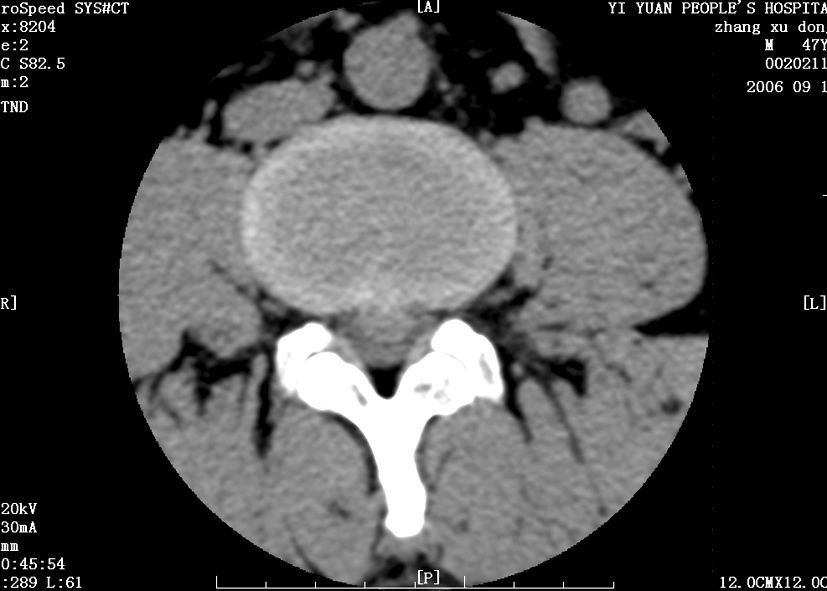
\includegraphics[width=.7\textwidth,height=\textheight,keepaspectratio]{./images/Image00470.jpg}
 \captionsetup{justification=centering}
 \caption{腰椎间盘突出\\{\small L\textsubscript{3/4} 椎间盘向后突出,并与椎间盘母体呈狭颈相连}}
 \label{fig23-7}
  \end{figure} 

此外,螺旋CT三维重建亦有助于椎间盘突出的诊断。

\textbf{【鉴别诊断】}

1.肿瘤:①椎间盘游离者需与占位性病变如转移瘤、淋巴瘤等相鉴别。但CT及CTM常鉴别困难。偶尔游离之碎片进入硬膜囊内似马尾肿瘤。②侧向型或过侧向型应注意与神经鞘瘤、神经根袖囊肿及大的神经根静脉丛鉴别。神经鞘瘤多伴有椎间孔扩大、神经根袖囊肿CTM可见造影剂充盈、神经根静脉丛可见增强有助于鉴别。

2.椎间盘疝块骨化与骨质增生:①骨化块内因含有未骨化的疝块组织故显示密度不均;而骨质增生密度均匀致密,轮廓亦多不规则。②骨化块旁有软组织密度影,提示为疝块。③以宽基底与椎体相连的骨化块,可见两者之间有间隙,并可见轻度硬化的骨皮质;而骨质增生的椎体后缘连线处常看不到间隙。以蒂样骨影连于椎体后缘的骨化块则不易误诊。④椎体后缘浅、小的骨缺损和硬化现象是诊断椎间盘突出并骨化的可靠征象。

3.术后复发与瘢痕组织:增强扫描诊断正确率达85%,表现为瘢痕组织呈明显强化;而椎间盘不强化。

\subsection{腰椎后缘软骨结节}

本病指发生于腰椎后缘突入椎体及椎管内的类圆形软骨结节,软骨结节即疝入椎体终板的椎间盘组织。大多为单发,偶尔多发。好发于L\textsubscript{4}
(70%),次为L\textsubscript{5} 和L\textsubscript{2} 。可与椎缘骨并存。

\textbf{【发病机制】}
曹来宾认为先天性解剖缺陷为因,慢性外伤起催化作用,骨内软骨结节是果,系与椎缘骨(也称为椎体前缘软骨结节)是同一病变,仅部位不同而已。实际上本病为椎体后缘的许莫氏结节。骨内软骨结节连同椎体后缘骨质可突入椎管,故常合并椎间盘后突。

\textbf{【临床表现】}
少数有外伤史,多发病于20~30岁。均有明显的腰腿痛,患侧直腿抬高试验阳性。

\textbf{【CT表现】}
①软骨结节:类圆形最多,还有不规则形、多囊状、长条状、裂隙状和三角形等(图\ref{fig23-8})。②软骨结节周围骨质硬化带:多存在,硬化带宽约7~9mm,密度多不均,边缘清楚;少数硬化带不明显,边缘欠清。③软骨结节后骨块:居椎体后缘正中或略偏于一侧,并突入椎管。骨块可游离,亦可与椎体相连;骨块大多单发,偶可多发呈碎片状。④椎体继发改变:可导致椎体相应的形态改变,主要表现为椎体终板向后膨出,致椎管矢状径变小及双侧隐窝狭窄。⑤多数可见同层椎间盘突出。

\begin{figure}[!htbp]
 \centering
 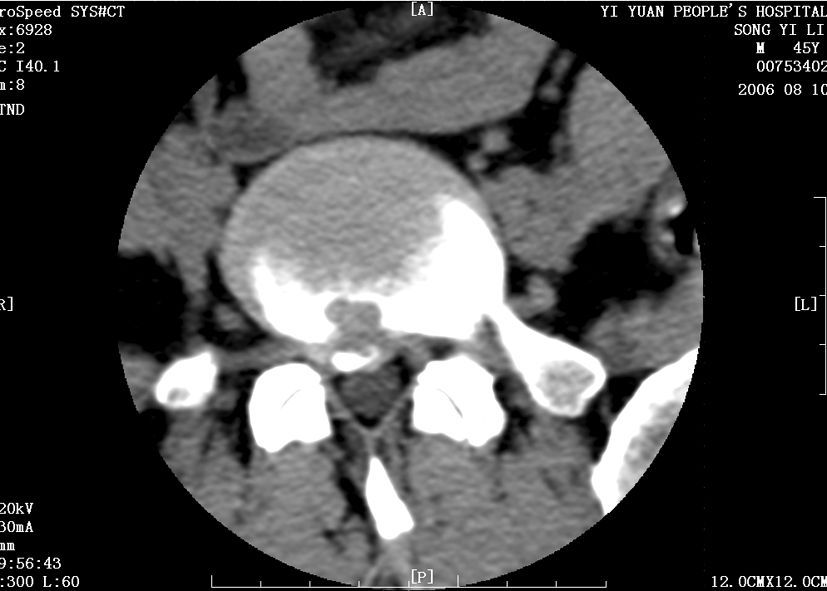
\includegraphics[width=.7\textwidth,height=\textheight,keepaspectratio]{./images/Image00471.jpg}
 \captionsetup{justification=centering}
 \caption{腰椎后缘软骨结节}
 \label{fig23-8}
  \end{figure} 

L\textsubscript{5}
椎体后下缘类圆形低密度结节,软骨结节后有骨块,同层椎间盘突出

\subsection{胸椎间盘突出}

\subsubsection{颈椎间盘突出}

多发于下颈段。与腰椎间盘突出相比,其中央型更多见,可能与颈椎椎体两侧的钩突关节限制有关。后突的间盘可压迫硬膜囊及颈髓,以致颈髓变形、萎缩,硬膜囊出现不同程度的梗阻(图\ref{fig23-9})。

\begin{figure}[!htbp]
 \centering
 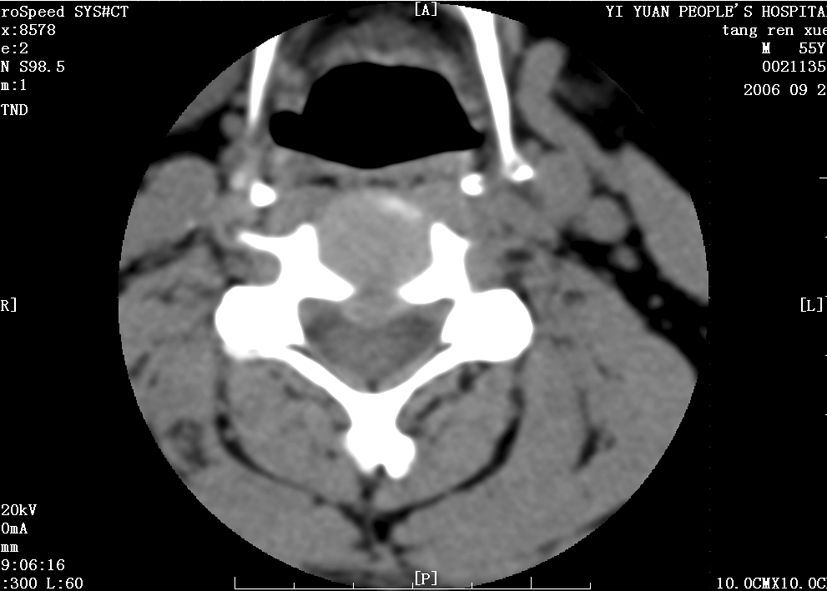
\includegraphics[width=.7\textwidth,height=\textheight,keepaspectratio]{./images/Image00472.jpg}
 \captionsetup{justification=centering}
 \caption{颈椎间盘突出\\{\small 显示椎间盘后突,明显超过椎体后缘}}
 \label{fig23-9}
  \end{figure} 

\subsubsection{胸椎间盘突出}

罕见,仅为所有椎间盘突出的1%。其CT表现与腰椎间盘突出相近。

\subsection{脊柱退行性骨关节病}

\textbf{【病理】}
首先为椎间盘及关节软骨的变性。椎间盘变性继发软骨下骨板增生硬化及椎体骨赘,还可见椎间盘突入椎体骨质形成Schmorl's(许莫氏)结节。关节软骨变性致使小关节增生。由于退行性改变,椎旁及关节韧带松弛,脊椎不稳、椎体前滑或后滑、小关节半脱位及黄韧带肥厚内褶。以上病变可导致椎管及椎间孔狭窄。

\textbf{【临床表现】}
可无明显症状,或只有颈、腰背部僵硬或(和)疼痛。并发椎间盘突出、椎管狭窄和脊椎滑脱时常压迫脊髓、神经根和血管引起相应的症状和体征。

\textbf{【影像学表现】}
①椎体上下骨板硬化及骨赘形成;②椎间盘退变表现如椎间隙变窄,椎间盘膨出、突出、钙化、“真空”现象以及许莫氏结节;③脊柱的韧带钙化或骨化,以黄韧带常见;④小关节退行性变征象;⑤脊柱曲度异常及脊柱不稳(退变性脊椎滑脱)。

\subsection{脊椎小关节退行性变}

本病所致的临床症状亦称为脊椎小关节综合征。好发于腰椎,单侧或双侧;也可见于颈、胸椎。见于一个或多个水平。X线平片不易显示,CT为最好的检查方法。

\textbf{【CT表现】}
①关节突增大,关节边缘骨赘(图\ref{fig23-10});②关节面增厚硬化,皮质骨与松质骨界限模糊,甚至关节突呈均匀硬化;③软骨下骨囊肿及骨糜烂;④关节间隙狭窄或关节半脱位,关节腔内出现“真空”(积气)表现;⑤关节囊及韧带钙化;⑥关节囊撕裂,破裂后出血及滑膜碎片等可进入黄韧带内和硬膜外间隙,以后发生钙化或形成滑膜囊肿;⑦上述关节病变可造成椎管中央部、侧隐窝或椎间孔狭窄。

\begin{figure}[!htbp]
 \centering
 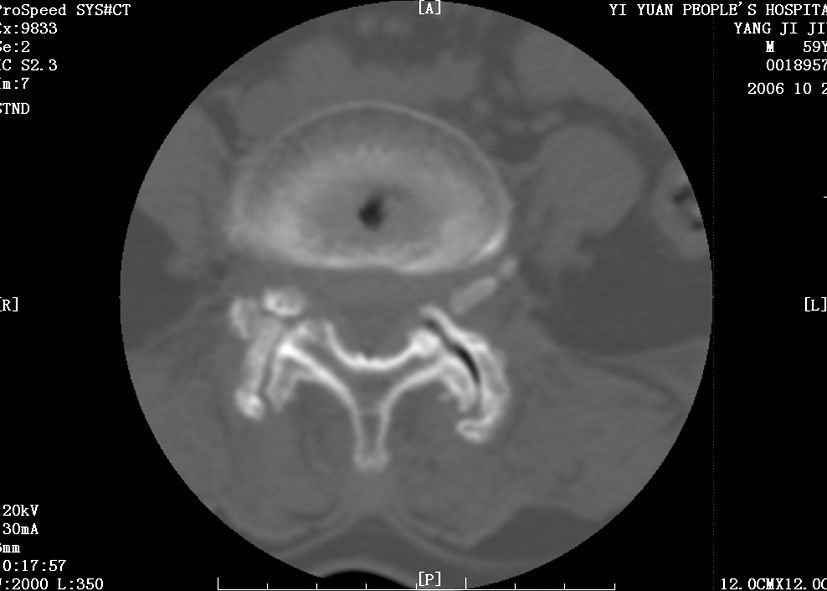
\includegraphics[width=.7\textwidth,height=\textheight,keepaspectratio]{./images/Image00473.jpg}
 \captionsetup{justification=centering}
 \caption{脊椎小关节退行性变\\{\small 左右侧关节突增大,关节边缘骨赘和游离骨片,关节面不规整,左侧关节内积气}}
 \label{fig23-10}
  \end{figure} 

但是,小关节退行性病变常累及几个关节,不一定引起小关节综合征,影像学不能判断病变与临床症状的关系。

\subsection{腰椎峡部裂}

椎弓崩裂之骨缺损多位于椎弓峡部(上下关节突间),亦可位于椎弓根、椎板。棘突、棘突旁者称为脊柱裂。

\textbf{【病因病机】}
其发生机理有先天性发育缺陷和创伤两种学说。一般认为椎弓峡部先天性发育缺陷或薄弱是发病基础,创伤是发病诱因。崩裂以L\textsubscript{5}
最常见,约占60%;L\textsubscript{4}
次之,约占30%;上腰部及下颈部亦可发生。多为双侧,多发峡部裂罕见。若伴椎体前移则称为真性脊椎滑脱。

\textbf{【临床表现】}
多见于20~40岁男性。最常见症状是下腰部进行性疼痛,可伴一侧或双侧下肢放射性疼痛。

\textbf{【CT表现】}

1.裂隙征:位于椎弓根偏后呈斜行、水平或略向前凸的裂隙状低密度影,边缘不规则。但边缘硬化,由致密骨质包绕,有助于与急性外伤所致的新鲜崩裂相鉴别(图\ref{fig23-11})。

\begin{figure}[!htbp]
 \centering
 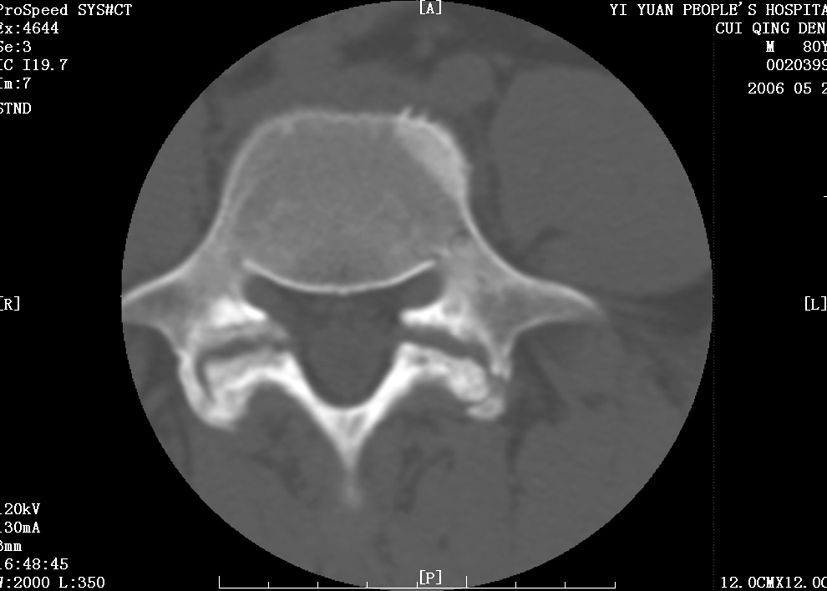
\includegraphics[width=.7\textwidth,height=\textheight,keepaspectratio]{./images/Image00474.jpg}
 \captionsetup{justification=centering}
 \caption{腰椎峡部裂\\{\small 双侧椎弓峡部均可见横行裂隙,边缘硬化}}
 \label{fig23-11}
  \end{figure} 

2.合并脊椎滑脱。

3.假性间盘突出征:此征是由于产生滑椎的上位椎体前移,而纤维环仍附着于下位椎体的终板上,当扫描该层面时,在其后缘可见椎间盘组织,而下位椎体后缘无类似影像。

4.双边征:是扫描线同时切及滑脱椎体相邻的两个椎体终板边缘所致的两道弧形高密度影。以后缘多见,亦可见于前缘。

5.游移征:此征只见于双侧裂者,是由于上位椎体的横向滑动所致。

6.磨旋征:可见于单侧裂或双侧裂。表现为棘突和椎体的扭曲、旋转以及两侧裂隙的不等宽。可与游移征并存。

7.其他:双关节征、椎管冗长、硬膜囊变形、裂隙周围增生或(和)碎骨块、软组织肿胀及退行性变表现。

\subsection{退变性脊椎滑脱}

一般将椎弓崩裂并椎体前移者称为真性脊椎滑脱。而由于随年龄增长椎间盘、小关节退行性变及周围韧带松弛等原因所引起的脊椎移位称为退变性脊椎滑脱。将退变性、化脓性、结核性等小关节病变所致的脊椎移位统称为假性脊椎滑脱。

\textbf{【病因病理】}
退变性脊椎滑脱的病因主要有:①椎间盘严重退变是老年人退变性脊椎滑脱的主要原因。正常腰椎屈伸运动轴中心紧靠髓核或在髓核内,当椎间盘突出或严重退变后,此轴后移,使屈伸运动在椎间小关节上产生“翘动”,导致椎间小关节退变,并引起腰椎失稳。②脊椎周围肌肉、韧带薄弱、松弛,也是导致脊椎不稳的重要因素。③腰椎小关节的不对称,使小关节易于退行性变,导致腰椎不稳。

退变性脊椎滑脱的椎弓保持完整,脊椎移位导致继发性椎管、椎间孔和侧隐窝狭窄。椎体移位导致或加重椎间关节退行性变。晚期椎间关节半脱位、关节变形、关节囊及黄韧带钙化或骨化。

\textbf{【临床表现】}
以60岁左右女性常见。临床症状和体征是由于椎间盘、椎间关节的退变及椎体移位引起的神经根和马尾受压所致。多首先表现为腰部不适,随之出现臀部和腰部疼痛、间歇性跛行,运动后加重。

\textbf{【CT表现】}
一般见于腰椎,以腰4、5多见;偶见于颈椎。本病80%为单发;80%以上为前滑,后滑、侧滑少见。CT可显示滑脱的部位和程度。由于椎体前移,造成上下椎体的相邻终板在同一层面上前后错位表现,呈现所谓“双终板征”。滑脱水平椎间盘多表现为退变、膨出。无椎弓峡部裂隙,均伴有椎间盘及小关节明显的退行性变(图\ref{fig23-12})。椎管变形、变小;椎间孔变形、变小;侧隐窝变窄。

\begin{figure}[!htbp]
 \centering
 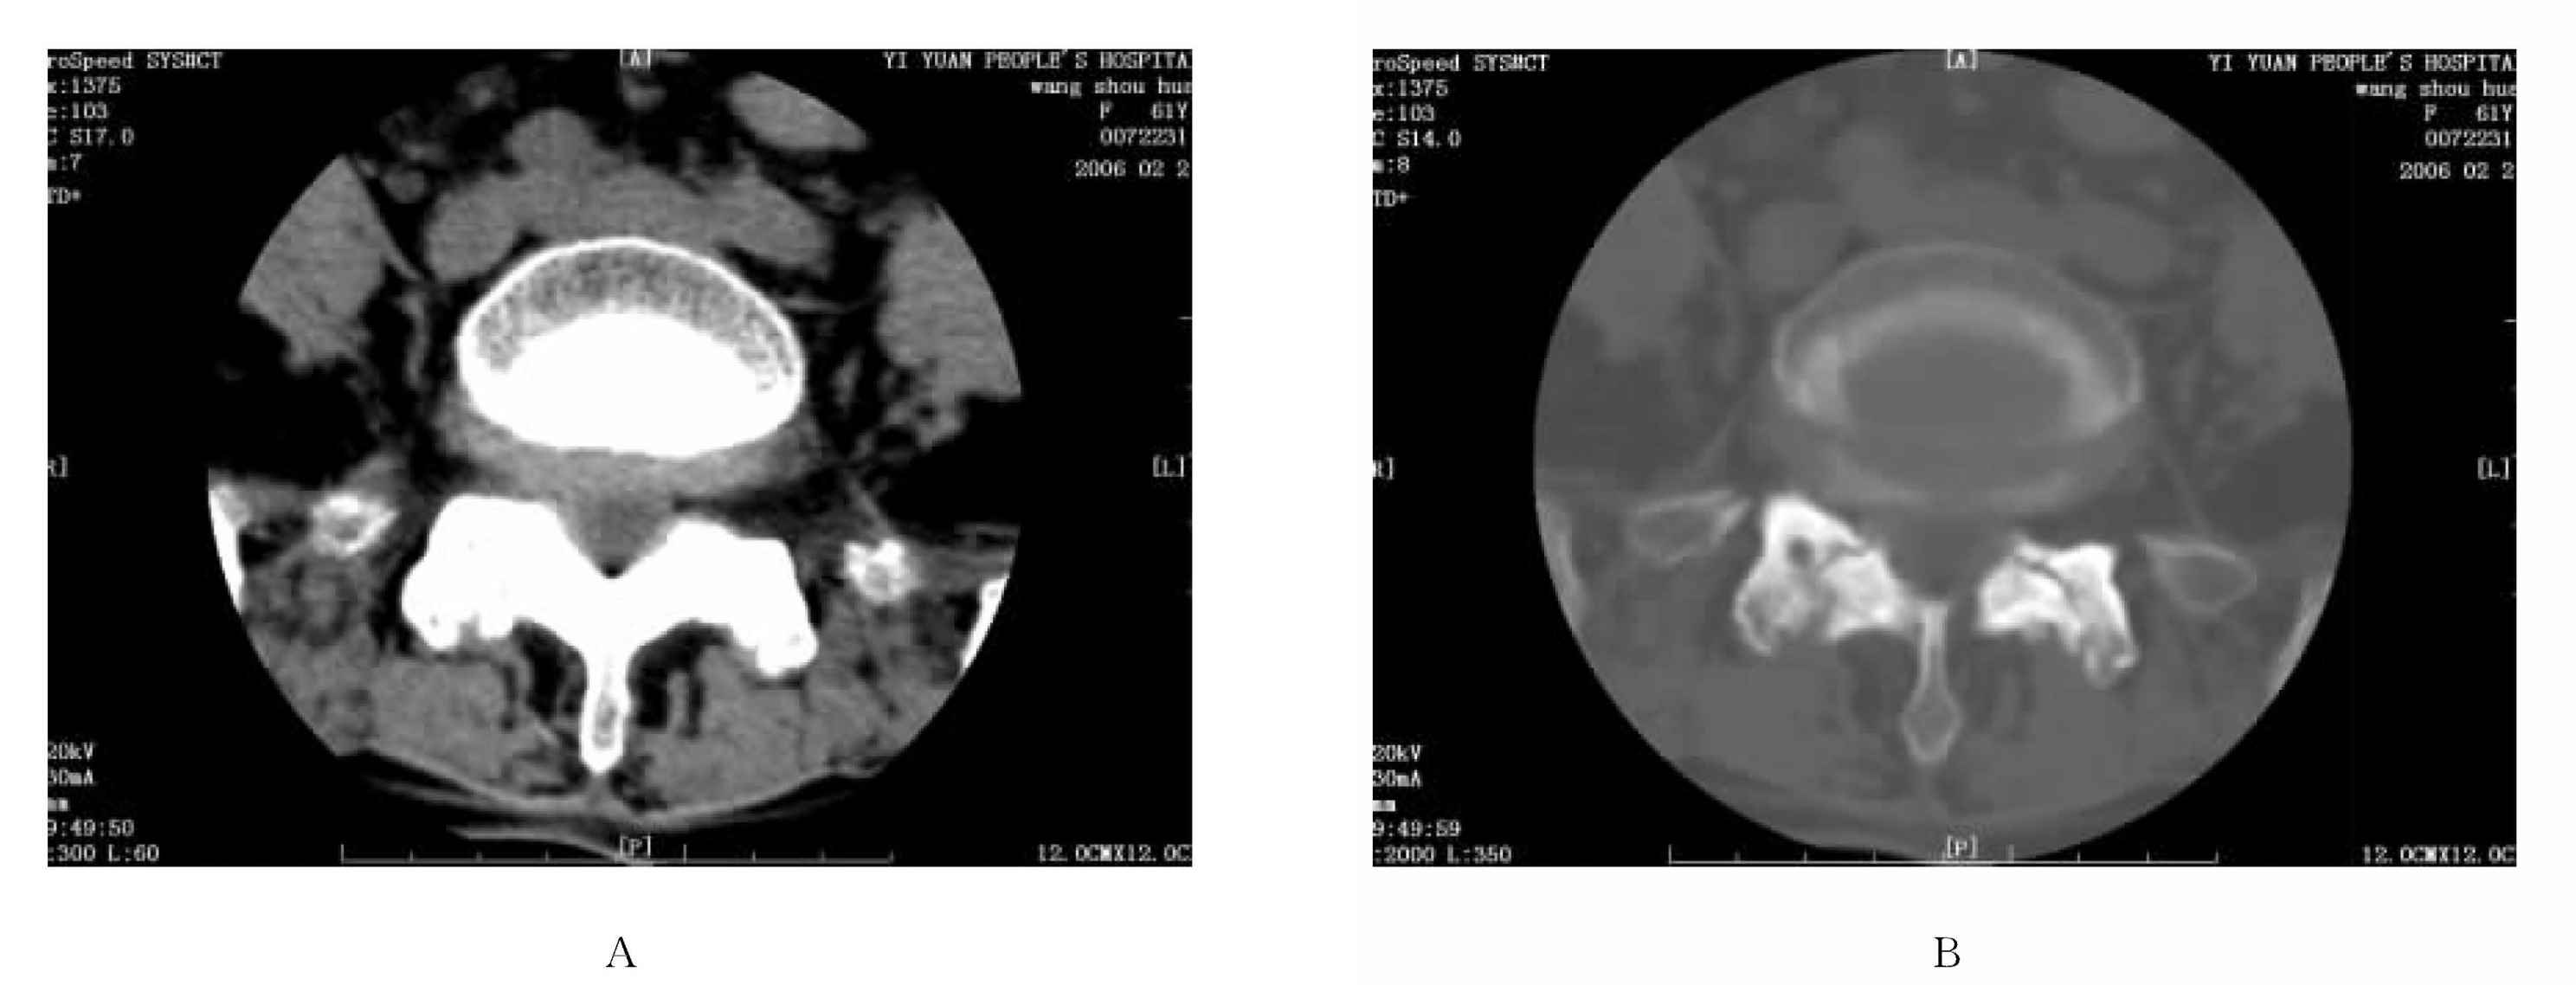
\includegraphics[width=.7\textwidth,height=\textheight,keepaspectratio]{./images/Image00475.jpg}
 \captionsetup{justification=centering}
 \caption{退变性脊椎滑脱\\{\small 有“双终板征”,并示小关节退变表现}}
 \label{fig23-12}
  \end{figure} 

\subsection{颈椎后纵韧带骨化}

后纵韧带骨化以颈椎多见,胸椎次之,腰椎少见,各部位可联合发生。10%颈椎后纵韧带骨化合并胸椎和(或)腰椎后纵韧带骨化。

\textbf{【临床表现】}
颈椎后纵韧带骨化主要见于黄种人。一般发生于壮年以后,以男性多见。轻者无症状,重者可产生脊髓、神经根受压表现。

\textbf{【CT表现】}
沿椎体后缘的骨化影,可呈圆形、半圆形、椭圆形或横条形等多种形态。骨化块内部可均匀或不均匀,其内可有低密度影。骨化块与椎体间有完整或不完整的条状间隙分开,常见到骨化块中间部与椎体后缘相连接,而两侧有间隙或切迹,可有硬膜囊或脊髓受压表现。

影像学类型:①连续型:条索状骨化跨越数个椎体节段,在椎间盘处略隆起。②间断型:在数个椎体后缘的点条状骨化,于椎间盘处中断。③局灶型:骨化影局限在椎间盘附近,位于变性或突出的椎间盘后方(图\ref{fig23-13})。④混合型:骨化在上颈椎多呈连续型,在下颈椎呈间断型。

\begin{figure}[!htbp]
 \centering
 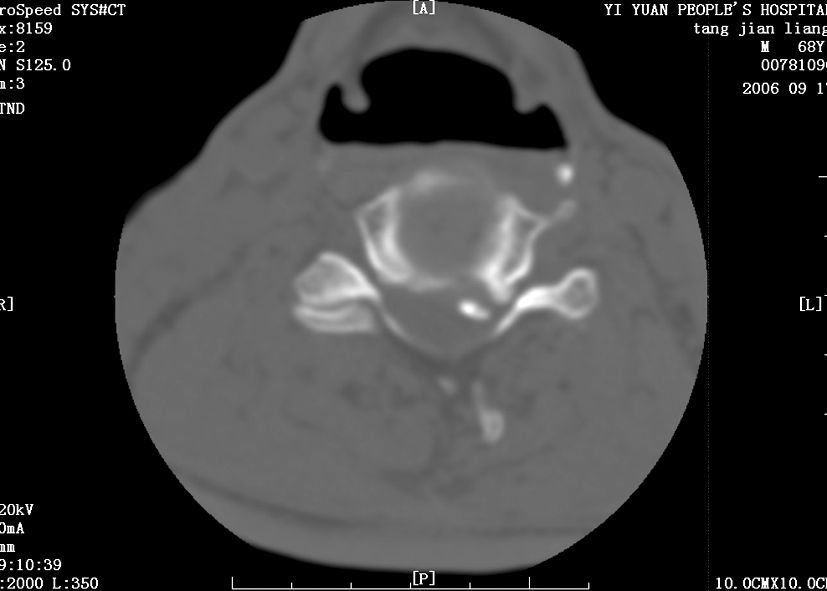
\includegraphics[width=.7\textwidth,height=\textheight,keepaspectratio]{./images/Image00476.jpg}
 \captionsetup{justification=centering}
 \caption{颈椎后纵韧带骨化\\{\small 突出椎间盘后方有局限性骨块}}
 \label{fig23-13}
  \end{figure} 

\subsection{胸椎后纵韧带骨化}

本病少见,发生率为0.6%,可合并颈椎后纵韧带骨化,通常还合并胸椎黄韧带骨化及弥漫性特发性骨增生症(DISH)。男性者几乎都伴有DISH。

\textbf{【临床表现】}
以女性多见,常无临床症状,可能是因骨化主要沿纵向发展而厚度无明显增加。但如骨化达一定厚度也会产生脊髓、神经根压迫症状。但也有报道,有患者骨化韧带厚度超过椎管矢状径的45%而无神经系统症状。

\textbf{【影像学分型】}
①桥型:范围局限,位于椎间盘后方,与相邻椎体连接成桥,常合并椎体前缘骨质增生,有时伴同水平的椎间盘突出。此型多单发或见于几个椎骨水平。②线型:呈线条样,常跨越几个椎体节段,与椎体间可有透亮间隙,不合并椎体的改变。③混合型:为上述两型的联合,多见于中上胸椎。

\subsection{黄韧带骨化}

本病好发于胸椎,以T\textsubscript{9} ~L\textsubscript{1} 节段多见。

\textbf{【病理】}
早期黄韧带内弹力纤维减少,胶原纤维增生,并出现透明变性,韧带弹性下降。脊柱后伸时韧带可出现折叠并突入椎管,并可造成微小损伤。在此基础上黄韧带逐渐增厚、钙化骨化。病变常见于黄韧带附着处。

\textbf{【临床表现】}
大约在20岁即可发生。单纯钙化常无脊髓、神经根受压症状,当其厚度超过5mm时,可有压迫症状。

\textbf{【CT表现】}
骨化最初发生于头侧或尾侧的附着点。前者沿小关节囊前缘和(或)椎管内面的线条形骨块,以关节囊前部多见;后者为椎板上缘的点条形骨块。可有硬膜囊或脊髓受压表现。

值得注意的是胸椎黄韧带骨化合并同水平后纵韧带骨化易造成严重脊髓压迫,应通过CTM或MR确诊其受压情况。

\subsection{弥漫性特发性骨增生症}

本病是一种原因不明的韧带骨化及骨质增生,可能与代谢或内分泌的变化有关,在病理上属退行性变。1971年Forestier比较全面的描述此病,把它与强直性脊柱炎及脊柱退行性骨关节病区分开来,因而此病被命名为Forestier氏病,亦称为强直性脊柱骨增生病。1975年,Resnick全面总结该病的X线表现(包括脊椎及四肢的病变),并命名为弥漫性特发性骨增生症(DISH)。

\textbf{【病理】}
肌腱及韧带附着处骨质增生及韧带骨化,发生在中轴骨及四肢骨。脊柱病变为以前纵韧带为主伴椎旁韧带的广泛增生骨化。骨盆及四肢关节的韧带附着处也可见骨质增生。

\textbf{【临床表现】}
发生于中老年人,男性发病居多,常为强壮或肥胖者,以及糖尿病患者。临床症状一般轻微,表现为腰背部僵直和疼痛,四肢关节痛及活动受限。临床症状轻微而X线征象显著为本病的特征。个别可出现脊髓、神经根受压表现。

\textbf{【影像学表现】}
X线平片是确立DISH的依据,主要X线特征为前纵韧带广泛骨化及韧带附着处的椎体前面骨质增生。好发于胸腰段及上胸椎,其次是颈椎。CT扫描可进一步观察是否合并后纵韧带骨化及硬膜囊脊髓是否受压、椎管是否狭窄。

1.胸腰椎:为前纵韧带及侧方韧带骨化,前者显著,常连续3个以上椎体高度,边缘呈波浪状;骨化韧带与椎体间有透亮带。少数并后纵韧带骨化。小关节及骶髂关节不受累,间隙不狭窄。

2.颈椎:①椎体前缘长条形及块状骨化、椎体边缘骨赘,若前突可压迫食管;②25%可合并后纵韧带骨化;③椎体后缘可见平滑的骨质硬化。

3.骨盆、跟骨、尺骨鹰嘴、髂骨及其他部位可表现为肌腱、韧带骨化及其附着点的骨质增生。

\textbf{【鉴别诊断】}

1.强直性脊柱炎:多见于青年男性。骶髂关节及脊柱小关节受侵犯,椎体韧带骨化薄而平滑,两者不难鉴别。

2.脊柱退行性骨关节病:无广泛的前纵韧带及侧方韧带骨化,值得注意的是两者可同时发生。

3.氟骨症:除骨质增生及韧带骨化外,尚有密度改变即密度增高、骨质软化或骨质疏松等,结合临床不难鉴别。

\subsection{椎管狭窄症}

本病即指由于椎管或椎间孔有效容积减小,压迫脊髓、神经根和血管等结构而引起的一系列症状和体征。椎管狭窄最常发生于腰椎,颈椎次之,胸椎少见,有的颈、腰椎同时受累。

\textbf{【病理】}

1.临床分类:①先天性:为出生时或出生后椎弓发育障碍造成椎弓狭窄,包括全身性骨发育障碍(如软骨发育不全、黏多糖病、脊柱骨骺发育不全、Down's综合征等)、合并脊椎畸形的先天性畸形,以及仅限于椎弓的发育障碍等,后者又称为发育性或特发性椎管狭窄。②后天性:见于多种原因,如退行性变、骨折及脱位、手术后、滑椎、氟骨症、Pget病、肢端肥大症、强直性脊柱炎、后纵韧带骨化、黄韧带肥厚、黄韧带骨化等。③混合性。

在先天性椎管狭窄中,以发育性椎管狭窄常见;在后天性椎管狭窄中,以脊柱退行性病变为主要原因,称为退行性椎管狭窄。发育性椎管狭窄一般都在发生退行性变后使椎管进一步狭窄才造成脊髓神经压迫,此时可称为混合性椎管狭窄。

2.解剖分类:①中央管狭窄:主要由于椎间盘突出或椎体后缘骨赘、后纵韧带骨化、黄韧带肥厚内褶、小关节骨赘、先天性椎板及小关节内聚、增厚等所致。②侧隐窝狭窄:主要由于小关节突增生肥大或椎间盘突出所致。③椎间孔狭窄:在胸、腰椎,神经根及脊神经节位于椎间孔上部,靠近上方的椎弓根下缘,小关节突增生肥大、椎体骨赘可能产生压迫症状;椎间盘膨出或突出只造成椎间孔下部狭窄,一般不压迫神经根。在颈椎,上述神经结构位于椎间孔下部,靠近下方神经根的上缘,产生压迫症状的常见原因是钩突增生;小关节突增生肥大造成椎间孔上部狭窄,只有在病变严重时才产生症状。造成椎间孔狭窄的其他原因有神经纤维瘤、脊椎前移症和手术后瘢痕组织增生等。

\textbf{【临床表现】}
临床上大多数椎管狭窄为获得性。单纯先天性发育狭窄可无症状,当继发骨质增生、椎间盘突出或韧带肥厚等因素时,才出现症状。

本病多于50~60岁出现症状,男性多于女性。病史较长、病情发展缓慢,呈渐进性发展。临床症状与脊髓、神经根、血管受压有关。①腰椎管狭窄表现为腰背痛、间歇跛行、下肢感觉运动障碍,站立行走或长时间固定一姿势时加重,休息或改变体位后症状减轻或消失。②颈椎管狭窄主要表现为颈后、肩背部疼痛,上肢无力及放射痛,有时伴下肢无力、走路不稳,严重者可发生四肢瘫痪、大小便失禁等。③胸椎管狭窄以T\textsubscript{8~11}
为多见,起病隐匿,早期症状为下肢麻木、无力,随病情加重可出现脊髓半切或横贯性损害表现。

\textbf{【CT表现】}
CT椎管测量的诊断标准国内外均不统一,而且个体差异甚大。本病的诊断应密切结合临床。虽然有肯定的狭窄存在,并非一定产生症状,这与病变的发展急缓及机体的适应力有关。综合众多学者意见,可采用下列标准。

\subsubsection{径线测量法}

1.椎管有效矢状径:颈椎≤9mm为绝对狭窄,9~10mm者为相对狭窄;胸、腰椎≤10mm为绝对狭窄,10~12mm者为相对狭窄。所谓有效矢状径即有椎间盘膨出、突出或后纵韧带钙化等患者,应测量其有效的实际径线而非骨性椎管的径线(图\ref{fig23-14}A)。

2.侧隐窝前后径:自上关节突内侧点至椎体(或间盘)后缘的距离,<2mm为绝对狭窄,2~3mm为相对狭窄(图\ref{fig23-14}B)。

\begin{figure}[!htbp]
 \centering
 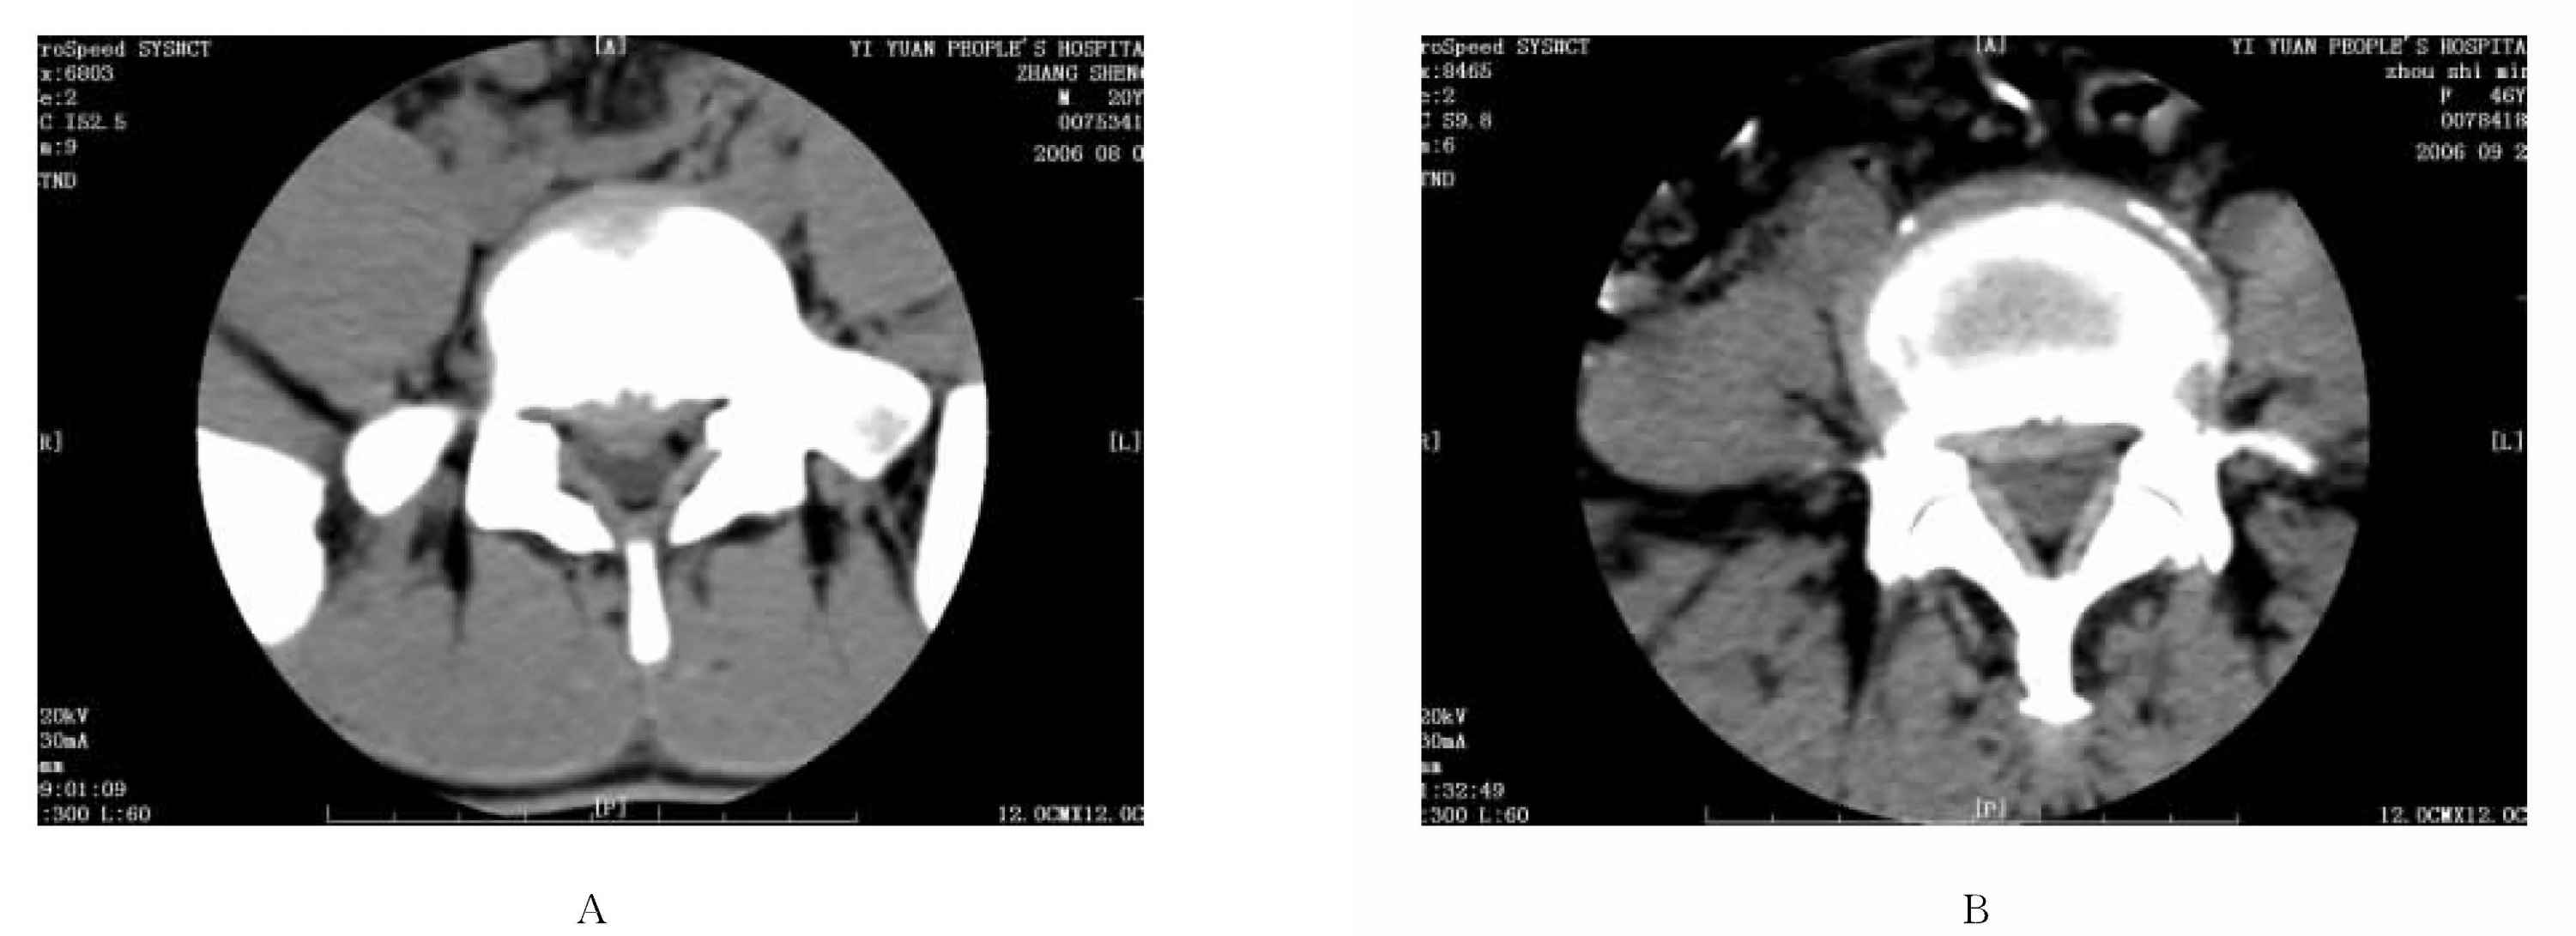
\includegraphics[width=.7\textwidth,height=\textheight,keepaspectratio]{./images/Image00477.jpg}
 \captionsetup{justification=centering}
 \caption{椎管狭窄症\\{\small A.腰椎间盘突出并中央管狭窄(前后径约0.8cm);B.腰椎间盘膨出并右侧侧隐窝狭窄(侧隐窝被间盘充填)}}
 \label{fig23-14}
  \end{figure} 

3.椎间孔高度:在腰椎<15mm则伴有神经压迫症状。还有人主张,在腰椎患侧椎间孔比健侧或上下椎间孔缩小50%以上时,才考虑为狭窄。但CT测量可靠性相对较差,不及平片。

\subsubsection{腰椎管狭窄面积测量法}

国外有学者认为,腰椎椎管矢状径对椎管狭窄的诊断符合率只有20%,只有硬膜囊横截面积≤100mm\textsuperscript{2}
时才能完全诊断腰椎管狭窄(即中央管狭窄),100~130mm\textsuperscript{2}
多为轻度狭窄。但这种方法不能对侧隐窝和椎间孔的狭窄做出评估。我们认为在测量面积时,因测量椎管的横截面比测量硬膜囊方便,且仍可以≤100mm\textsuperscript{2}
作为腰椎管狭窄的诊断标准。

此外,CT虽然有利于诊断三叶状狭窄变形的椎管,但由于解剖变异,正常情况下,特别在L\textsubscript{5}
平面三叶草形椎管亦可出现,故不能仅凭此征诊断椎管狭窄。应注意观察硬膜囊是否受压。

\subsection{椎间盘钙化}

\textbf{【病因】}
成人椎间盘钙化属退行性改变,钙化局限在一个或几个椎间盘,多发生在纤维环,无临床症状。广泛的钙化见于多种疾病,如褐黄病、假痛风、甲状旁腺功能亢进、肢端肥大症、淀粉样变、强直性脊柱炎、维生素D中毒等。儿童椎间盘钙化较少见,好发于颈椎,病因尚不肯定,可能与外伤、炎症或维生素D及钙代谢障碍有关。

\textbf{【CT表现】}
髓核钙化位于椎间盘中央或稍后的高密度影,密度均匀或不均匀;纤维环钙化发生在外周部分,呈分叶状。

\subsection{儿童钙化性椎间盘病}

本病习称儿童椎间盘钙化,由于病因未明,也被称为特发性椎间盘钙化。因本病累及髓核、纤维环和软骨板这一功能性整体并常发生椎体改变,亦称为儿童钙化性椎间盘病。

\textbf{【病因】}
病因尚不肯定,可能与外伤、炎症或维生素D及钙代谢障碍有关。本病钙化机理不明。

\textbf{【临床表现】}
本病男女发病相近。国外文献中从生后2小时至20岁患者近400例,70%为5~12岁儿童,平均7岁。本病以白种人多见,黑人和亚洲人罕见。有些患者出现发热和疼痛表现。本病属自限性良性病变,无特殊治疗,往往进行对症处理,多数患者在数周或数月后临床症状可完全消失。

\textbf{【影像学表现】}
以颈、胸段多见,腰段少见。可侵犯一个或多个椎间盘。①椎间盘钙化、髓核钙化:可呈团块状、盘状、碎裂状。②髓核脱出或移位:可产生神经压迫症状。③椎体改变:椎体变扁,前缘呈尖角状突出形成假性骨赘,椎体改变可能与疼痛相关。④脊柱曲度失常:以颈椎多见。

钙化发生或吸收的快慢差异很大,钙化在数周至数年内消失。胸段钙化消失较颈段者慢,无症状的钙化消失较有症状者慢。

\subsection{椎体内真空裂隙}

本病也称为椎体内真空现象。最早由Maldague于1978年提出,指在骨折的椎体内出现气体影。

\textbf{【病因病理】}
绝大多数发生于骨质疏松性骨折的椎体(包括原发性和继发性骨质疏松症),少数发生于肿瘤(多为多发性骨髓瘤)所致的病理骨折。此外,脊柱骨髓炎、结核、椎体许莫氏结节等亦偶尔在椎体内出现气体影。

多认为该现象是椎体缺血坏死的特征性表现。可能是由于椎体血管损伤、受压或栓塞,导致椎体血供减少,甚至中断。缺血坏死的椎体出现压缩骨折,形成椎体内裂隙。裂隙内压力下降,出现负压时,溶解在体液内的气体逸出,形成椎体内真空征象。还有人认为椎间盘内的气体可通过骨折的终板进入椎体内形成该现象。

\textbf{【影像学表现】}
①以胸、腰段多见,压缩较明显的椎体易出现,气体位于椎体压缩骨折的部位,多靠近终板。②X线呈横行线状气体影,1~3mm高,边缘有硬化,少数呈圆形;CT横断像气体影外形规则。该征象可存在数月或数年,然后自行消失。③椎体许莫氏结节内含有的气体多为垂直走行或圆形,相邻近的间盘内可有积气、椎体终板有缺损,可与其他原因所致者鉴别。

\section{椎管内结构损伤}

\subsection{硬膜囊撕裂和神经根断裂}

\subsubsection{硬膜囊撕裂}

当其破裂时,CTM示注入的造影剂外溢到椎管内,硬膜囊轮廓模糊。

\subsubsection{神经根撕裂}

多发生于C\textsubscript{7} 和T\textsubscript{1}
,常由于上臂外展造成。CTM表现为神经根鞘充满造影剂突入椎间孔,鞘内无神经根影,硬膜囊可稍向对侧移位。

\subsection{急性脊髓外伤}

本病是一种严重的外伤,占全身损伤的0.2%~0.5%,在脊柱骨折中伴发脊髓损伤者占20%。

\textbf{【病因病理】}
工伤、车祸、运动及火器伤是其主要原因。闭合性脊髓外伤主要来自骨折碎骨块、脱位椎体的压迫,外伤性椎间盘的压迫和末梢穿动脉的阻塞也是其重要原因。脊髓外伤病理上按损伤轻重分为脊髓震荡、脊髓挫裂伤、脊髓压迫或横断、椎管内血肿。

\textbf{【临床表现】}
脊髓损伤的早期阶段主要表现为脊髓休克。如系脊髓震荡则短期内(2周)可恢复正常;脊髓挫伤或部分挫断时,其损伤平面以下的运动和感觉均消失。

\textbf{【CT表现】}
脊髓外伤最常累及颈髓、胸腰段脊髓。脊髓震荡伤多无阳性发现。

1.脊髓挫裂伤和水肿:脊髓外形膨大、边缘模糊,髓内密度不均,有时可见点状高密度灶,局部蛛网膜下腔变窄,但水肿较轻时上述改变不明显。

2.脊髓断裂:CTM示多合并硬膜囊破裂,造影剂充满硬膜内外整个椎管;硬膜囊中心的脊髓影可变形。如完全断裂,脊髓影则消失。损伤上下的正常段仍可见充盈造影剂的硬膜囊和中间的脊髓。

\subsection{椎管内血肿}

\textbf{【病因病理】}
椎管内血肿可分为创伤性和自发性两类。病理上有硬膜外、硬膜下、脊髓内、蛛网膜下腔之分,但硬膜下较少;蛛网膜下腔由于脑脊液的流动,罕有血肿形成。

\textbf{【临床表现】}
可有颈或胸部刺痛,随即截瘫,病情呈急性或亚急性进展。疼痛部位大多局限,并与出血部位大致相同,但由于牵涉痛和神经根放射痛,疼痛部位可较弥漫。

\textbf{【CT表现】}

1.硬膜外血肿:平扫表现为紧贴椎管壁的局限性或包围整个硬膜囊的高密度影,界限清楚。①硬膜外脂肪消失,被血肿替代,血肿呈新月形或弧形,CT值为50~90Hu,血肿与邻近的骨结构直接相连,相应硬膜囊受压变形。②血肿好位于后外侧,可能与后外侧硬膜外间隙较宽有关。③由于该间隙前外侧有神经根出入椎间孔,较固定,故后外侧的血肿易于纵向蔓延。有时可经椎间孔向外蔓延。但上方不能进入颅内,是因硬脊膜紧密附着于枕骨大孔缘。

2.硬膜下血肿:类似CTM所见,这时的高密度影不是造影剂,而是新鲜血液。血肿与邻近骨结构不直接相连,而有硬膜外脂肪间隙相隔,血肿亦不会沿椎间孔向外蔓延。

3.脊髓内血肿:脊髓内出现外形不规则、界限模糊的高密度区。

但在血肿吸收期,上述3类血肿难以显示和明确诊断。

\subsection{慢性脊髓外伤}

\textbf{【病理】}
慢性脊髓外伤分别表现为脊髓囊变、空洞、萎缩、软化、栓系及慢性受压6种病变。脊髓囊变与脊髓瞬间压迫伤有关,其病变局限。脊髓空洞、萎缩均与脊髓持续受压有关,病变潜在进展,其中脊髓萎缩主要与缺血引起脱髓鞘有关。脊髓软化可能由伤后脊髓缺血引起。脊髓栓系是伤后蛛网膜粘连所致。

\textbf{【影像学表现】}
以MR检查为优,CT亦可提供一定的诊断依据。①脊髓囊变:髓内局限性、边缘锐利的水样密度灶。②脊髓软化:MR表现为病变段脊髓边缘模糊,呈形态不规则的异常信号区,亦有学者将脊髓囊变归入脊髓软化中。③脊髓萎缩:MR诊断标准尚不统一。国外有学者把颈髓前后径<6mm或7mm视为萎缩;胸髓前后径<6mm视为萎缩。脊髓萎缩并不在损伤处最明显。④脊髓空洞(见本章第三节)。⑤脊髓栓系:少见,脊髓与蛛网膜粘连固定于椎管壁使脊髓移位、紧张、变性,功能缺失。脊髓后移和外伤性椎间盘突出均能造成脊髓后移紧贴椎管壁,但这并不符合栓系的诊断;无脊髓受压的脊髓粘连且伴脊髓功能缺失,才可诊断为栓系。⑥脊髓慢性受压:可由碎骨片、脊柱后突成角及椎间盘突出引起,一般有继发改变如脊髓空洞、软化和萎缩。

\subsection{脊髓萎缩}

\textbf{【病因病理】}
本病是脊髓组织的变性退化改变,其原因很多,如外伤、多发性硬化、血管畸形、肌萎缩性脊髓侧索硬化、脊前动脉闭塞、脊髓炎性病变等。病理主要表现为脊髓变细,常局限于几个节段,少数可累及脊髓全长。

\textbf{【临床表现】} 主要表现为相应脊髓平面的运动、感觉异常。

\textbf{【CT表现】}
CTM可见脊髓变细、边缘光滑,密度多无改变;蛛网膜下腔相对变大。正常颈膨大前后径为0.8cm,左右径为1.3cm;胸髓最窄处前后径为0.6cm,左右径为0.8cm。因此,当颈膨大<0.6cm×1.1cm,胸髓<0.5cm×0.6cm时,即可提示脊髓萎缩。

\section{椎间盘及椎管内感染性疾病}

\subsection{椎间盘炎}

本病亦称为椎间盘化脓性感染、化脓性椎间盘炎、椎间盘感染,为少见病。广义而言椎间盘炎可归入感染性脊椎炎的范畴。

\textbf{【病因】}
致病菌为革兰氏阳性或阴性菌,最多见的是金黄色葡萄球菌(约占84%),其次为大肠杆菌,免疫低下病人还可感染真菌,有时为多种细菌混合感染。

1.原发性:为经血液循环将细菌带入椎间盘。有以下几种途径:①致病菌经血液循环进入终板下松质骨后再侵犯椎间盘。发育中的椎体动脉主要分布在前侧,进入后侧的血流较少,所以前侧易发病。②经血液循环直接进入椎间盘。儿童椎间盘血供较多,细菌可直接经血液循环进入椎间盘,故儿童可以先引起椎间盘感染,再破坏相邻椎体终板,这是儿童多为原发性的原因之一。成年后椎间盘血供消失,但因其退变而有肉芽组织长入,细菌可经肉芽组织进入椎间盘。③经Batson静脉系统进入椎间盘,该静脉丛位于椎管内,无瓣膜,与椎间盘紧密相邻,可沟通椎体与骨盆内等椎体外静脉丛。

2.继发性:为手术、椎间盘穿刺、开放性外伤等,将细菌直接带入椎间盘。

\textbf{【病理】}
主要包括椎间盘水肿、液化坏死、终板破坏,邻近椎体骨质疏松、破坏等,还可在硬膜外、椎旁软组织形成脓肿或蜂窝组织炎。

\textbf{【临床表现】}
病人症状可剧烈,迅速恶化甚至致死,也可轻微缓慢。血液或椎间盘标本未能培养出细菌者临床表现多轻微。原发性者多见于儿童,少见。继发性者多见于成人。

1.儿童型:年龄多在1~15岁,男女之比约2∶1。最常见的症状为背痛、跛行、肌肉痉挛,行走久立后加重,可有呼吸道、胃肠道、耳或泌尿系感染的前期表现。主要体征为脊柱局部压痛、叩击痛和活动受限。有的体征可类似神经肌肉病变、化脓性关节炎、阑尾炎、尿路感染、脑膜炎或骨髓炎等,多预后良好。

2.成人型:年龄平均56岁,男女之比约为2∶1。①原发性者常发病缓慢,偶有急性发病。多体温正常或低热、个别高达39℃以上。最常见症状为下腰痛,活动后加重;体征为脊柱局部压痛、叩击痛和活动受限,一般预后好。②继发性:上述临床症状较重,截瘫和死亡率均较高,多有手术指征。

3.实验室检查:血沉增快为本病的一大特点。有学者报道椎间盘术后2周腰痛加剧、血沉高于50mm/h,应考虑为术后椎间盘炎。血培养细菌阳性率不高;椎间盘穿刺活检培养比血培养阳性率高些,但儿童型也有50%~70%为阴性。白细胞多数不高。细菌感染时C反应蛋白阳性率可达80%~100%。

\textbf{【影像学表现】}

1.平片表现:①原发性:发病后2~4周惟一的表现为椎间盘变窄,高度可降至50%以上。一般均可见到,但病灶局限者椎间盘变窄可不明显。随后出现终板脱钙和(或)不规则,同时可出现相邻椎体边缘的不规则硬化。有时可见明显骨质破坏,多开始于椎体前部即“干骺部”骨髓炎。破坏形式有磨角状、波浪状、虫蚀状和溶骨状,累及椎体的高度均在40%以下。随访可见椎间隙进一步变窄,骨质增生硬化明显,骨赘、骨桥形成,脊椎后突、侧弯畸形等改变,但椎体一般不融合。②继发性:与原发性表现相似,但有文献报道易引起溶骨性破坏,椎体破坏、硬化更显著而广泛。一般术后1~3个月出现骨质破坏及骨质硬化。

2.CT表现:在发现椎体骨质破坏、硬膜外脓肿和脊髓受压方面较平片敏感。①早期主要表现为椎间盘密度减低、且变扁变大,类似椎间盘膨隆征象,有时密度明显减低如掏空状。病变椎间盘与腰大肌之间界限模糊。②随后可见椎体前部软骨终板下不规则骨质破坏及增生改变。③多见椎体前侧缘宽约3mm的弧形软组织影,与腰大肌间有脂肪间隙存在。但也偶可表现为腰大肌区大脓肿,而与结核难以鉴别。总之,当发现上述椎间盘改变,又无明显脓肿形成时,应考虑到椎间盘炎可能。

\textbf{【鉴别诊断】}

1.脊柱化脓性骨髓炎:关于椎间盘炎与脊柱化脓性骨髓炎的关系和命名尚有争论。有学者认为尽管平片上早期椎间隙变窄,而MR已显示有邻近椎体的炎症改变,主张命名为化脓性感染性脊椎炎,将椎间盘炎和脊椎化脓性骨髓炎都包括在内。但很多学者认为当炎症主要侵犯椎间盘时,即称为椎间盘炎。

椎间盘炎一般在早期特征性出现椎间隙变窄,破坏椎体的高度较小;而脊椎化脓性骨髓炎则主要累及椎体,很少或不累及椎间盘。

2.结核:以前常将椎间盘炎误诊为边缘性结核。①结核起病缓慢,病程长,以月、年计算;而椎间盘炎临床症状较急,继发性者可有相应病史,可有高热,在2~4周内即出现典型的椎间隙变窄。②结核引起的局部疼痛和叩击痛一般较轻,甚至无明显疼痛,仅感不适;而椎间盘炎均有明显的疼痛和叩击痛。③结核的椎体骨质破坏明显,常楔形变;而椎间盘炎不造成椎体的楔形变。④结核的椎旁脓肿范围较大;而椎间盘炎常较小。⑤椎间盘炎常有自限性;而结核为进行性骨质破坏。⑥结核CT常呈特征性的碎裂状改变,没有硬化;而椎间盘炎可见确切的破坏灶,其边缘明显硬化。⑦平片显示骨赘形成及椎体终板的硬化为椎间盘炎特征性改变;而结核除非后期或合并化脓性感染没有这些改变。

3.巨大许莫氏结节:为椎间盘物质突破软骨终板及骨性终板陷入椎体骨质内,而形成较大凹陷,其周围反应性骨硬化,椎间隙可变窄。但无侵蚀样骨质破坏及周围软组织肿胀。

\subsection{椎管内硬膜外和硬膜下脓肿}

椎管内脓肿一般是指椎管内急性化脓性感染,以硬膜外脓肿最常见,硬膜下较少见,脊髓内极为少见。

\textbf{【病因病理】}
病原菌以金黄色葡萄球菌为多,常由邻近组织直接蔓延而来,也可由远处感染灶经血液迁徙而来。病原菌在硬膜外间隙扩散,形成蜂窝组织炎,最终形成脓肿。脓液主要集聚于硬膜囊的背外侧,上下可延及数个脊髓节段,有时可达椎管全长。脓肿吸收后可形成肉芽肿,并因脊髓的受压或血循环障碍而导致脊髓实质的缺血、水肿和软化等。

\textbf{【临床表现】}
亚急性脓肿最为多见。起病时有高热、寒颤、WBC增高等全身感染表现,以后出现脊背疼痛、脊柱活动受限,进而出现脊髓功能损害症状。

\textbf{【CT表现】}

1.硬膜外脓肿:表现为硬膜外密度增高,正常血管、神经结构模糊。亚急性或慢性脓肿可见到密度更高的肉芽组织,邻近骨质可有轻度增生或不规则破坏,有时可见硬膜囊及神经根鞘增厚。

2.硬膜下脓肿:表现为硬膜囊不规则变形,密度不均匀增高。此外,CTM更有利于脓肿的显示。

\subsection{椎管内肉芽肿}

\textbf{【病因病理】}
肉芽肿是由新生的成纤维细胞、毛细血管及数量不等的炎性细胞组成的幼稚结缔组织。可分为两类:①感染性:化脓细菌性、结核性、梅毒性、真菌性、寄生虫性肉芽肿以及非特异性炎症性肉芽肿。②非感染性:主要是异物残留所致,亦可为化学药物性刺激所致(如国内有椎管内干细胞移植治疗后产生肉芽肿的报道)。

\textbf{【临床表现】}
主要表现为肌力下降、肌肉萎缩,以及感觉异常、括约肌功能障碍等。

\textbf{【影像学表现】}
肉芽肿的显示MR优于CT,可见充满椎管内的异常密度灶或异常信号,硬膜囊可受压;增强扫描可见轻度不均匀强化,一般无明显坏死囊变。需结合病史综合诊断。

\subsection{脊膜炎和脊髓炎}

\subsubsection{脊膜炎}

多并发于脑膜炎,常见于细菌感染,如肺炎双球菌、结核杆菌,真菌、病毒性少见。

\textbf{【CT表现】}
由于骨伪影的干扰,多无阳性发现。蛛网膜炎的CTM表现为脊髓偏于硬膜囊一侧,或神经根聚集在一起。有时神经根贴于增厚的蛛网膜壁上,呈现硬膜囊内空虚,硬膜囊变小或不规则。严重时蛛网膜下腔可完全阻塞。

\subsubsection{脊髓炎}

多见于病毒感染,如疱疹病毒、柯萨奇病毒、脊髓灰质炎病毒等,病变多累及脊髓灰质。脊髓炎也可由硬膜外脓肿、结核或真菌性脑膜炎蔓延而来。

\textbf{【CT表现】}
由于脊髓的外形变化轻微,仅少数可见脊髓增粗,CT及CTM多无阳性所见,偶见脊髓梭形增粗,似髓内占位表现。

总之,CT对上述两者的诊断无特异性,对病变的显示不及MR。

\subsection{放射性脊髓炎}

放射治疗如脊髓暴露在放射野内,有可能发生轻重不一的急性或慢性放射性脊髓炎,并导致各种严重并发症。

\textbf{【病理】}
①早期主要表现为脊髓充血、水肿、脱髓鞘以及神经细胞变性等改变。②晚期主要为脊髓发生坏死、液化、囊变、胶质细胞增生及继发萎缩等改变。

\textbf{【影像学表现】}
MR有助于上述病理改变的显示。CT难以显示脊髓所发生的放射性病理改变,故诊断价值不大。

\section{椎管内血管疾病}

\subsection{椎管内血管畸形}

椎管内血管疾病包括血管畸形、动脉瘤、海绵状血管瘤与梗死等。椎管内血管畸形是指脊髓血管先天性发育异常而形成的一类病变,约占脊髓疾病的3.3%~12.5%。可发生于脊髓各个节段,脊髓内外可同时受累,颈、胸段血管畸形以髓内病变为主,腰段则多位于脊髓后方。

\textbf{【病理】}
畸形血管可引起脊髓受压、缺血、出血或血栓形成。根据异常血管的形态和结构,可将血管畸形分为4类。

1.动静脉畸形:该类最常见。由供血动脉、畸形血管团和引流静脉组成;好发于胸腰段,其次为胸段、颈段。又可分为以下两大类:

(1)硬膜内动静脉畸形:①球型动静脉畸形:位于髓内,由小的迂曲血管构成球状血管团,但畸形血管之间无脊髓组织存在;②幼稚型动静脉畸形:血管团亦位于髓内,血流迅速,在畸形血管团的间隙中可看到脊髓组织;③动静脉瘘:无异常血管团,在脊髓内或其表面形成动静脉直接短路。上述球型和幼稚型均由脊髓前动脉供血,回流静脉明显扩张,沿脊髓背侧走行,汇入硬膜外静脉丛。

(2)硬膜外动静脉畸形:由肋间动脉发出的硬膜动脉供血,经脊髓静脉回流入脊髓背侧的冠状静脉丛,血液回流较缓慢。

此外,约20%脊髓动静脉畸形合并有动脉瘤。动脉瘤多为囊状,70%发生于脊髓腹侧,颈段与胸段脊髓约各占一半。

2.静脉畸形:由曲张的静脉团组成,常伴血栓形成。

3.动脉畸形:由多条动脉集聚而成,常位于脊髓表面。

4.毛细血管扩张症:由大小不一扩张的毛细血管组成,多位于脊髓后索。

\textbf{【临床表现】}
可见于儿童和青壮年等,多起病突然,也可缓慢起病。症状加重和自行缓解交替出现,常以疼痛(病变部位神经根分布区)起病,随后出现肢体无力、感觉异常,以及括约肌功能障碍(大小便功能障碍)。如有出血可出现急性脊髓横断症状。

\textbf{【CT表现】}

1.平扫:病变部位脊髓局限增粗,有时在其表面可见斑点状钙化灶。

2.增强扫描:静脉注射造影剂后在脊髓内或其表面可见到异常强化、扩张的血管,呈迂曲走行、多环状或团块状分布,其周围有时可见粗大的供血动脉及引流静脉。病灶多位于脊髓背外侧;颈胸段病变范围较大,腰段多较局限。动态扫描畸形血管的密度与正常血管多同步升高并迅速降低。

3.CTM表现:脊髓表面点、条状边缘光滑的充盈缺损。伴有出血时可见到高密度血肿,脊髓横径增宽。畸形血管内血栓形成时,相应脊髓呈萎缩改变。

\subsection{腰椎椎间静脉压迫症}

本病是指椎间静脉由于不同原因受压迫后,导致椎间静脉远心端及椎管内前椎内静脉丛的血液回流不畅,发生扩张和曲张,压迫神经根而产生临床症状。

\textbf{【腰椎间静脉的解剖】}
在腰椎椎管内,从脊髓出来的静脉随脊神经根穿过硬膜注入硬膜外腔的椎内静脉丛,该静脉丛分为前、后两组。后组发育较差,前组在椎体、椎间盘的后面及后纵韧带的两侧,与位于椎弓和黄韧带前方的后椎内静脉丛之间有吻合支相连,然后汇入位于椎间孔内的椎间静脉。椎间静脉位于椎间孔上部,出椎间孔汇入腰升静脉。

\textbf{【病因】}
①先天性:包括椎间静脉发育不良出现狭窄或在椎间孔内走行异常、受相邻的神经或纤维隔压迫产生迂曲扩张,还有罕见的动静脉畸形或动静脉瘘产生的压迫。②后天性:多见,多由于脱出的椎间盘、小关节或腰椎椎体后缘的骨质增生或增厚的黄韧带等对椎间静脉的压迫。

此外,少数情况下由于静脉系统内无瓣膜存在,可因心衰或门静脉高压引起胸腔或腹腔内压力增高,导致椎间静脉或前椎内静脉丛代偿性扩张或曲张。

\textbf{【临床表现】}
多见于青壮年。其临床症状无特异性,有慢性腰腿痛病史,或有坐骨神经痛病史。与椎间盘突出、黄韧带肥厚、椎间小关节退变和神经根管狭窄所产生的症状相似,难以鉴别。

\textbf{【CT表现】} 本病多发生于L\textsubscript{4} /L\textsubscript{5}
或L\textsubscript{5} /S\textsubscript{1} 平面,其CT表现如下。

1.直接表现:受压迫的椎间静脉远侧扩张增粗,同层面常可见到椎体后缘骨质增生、小关节骨质增生或椎间盘突出到椎间孔等。

2.间接表现:直接流入椎间静脉的前椎内静脉丛呈不同程度的扩张或曲张的血管影。位于硬膜囊的前方、左前或右前方,以及椎间孔内。其形态为弯曲的条形、环形或混合存在。

扩张的椎间静脉或前椎内静脉丛的直径为2~5mm,以2~3mm者多见,增强扫描更加有利于对曲张血管的显示。此外,还可见到硬膜囊前缘受压变形,硬膜囊前方、左前、右前和椎间孔内脂肪间隙变窄或消失。

\section{椎管内肿瘤}

\subsection{概述}

椎管内肿瘤包括发生于椎管内各种组织的原发性(见表\ref{tab23-1})和继发性肿瘤。人群发生率为(0.9~2.5)/10万。临床上根据肿瘤的发生部位可分为4类。

\begin{table}[htbp]
\centering
\caption{椎管内原发性肿瘤}
\label{tab23-1}
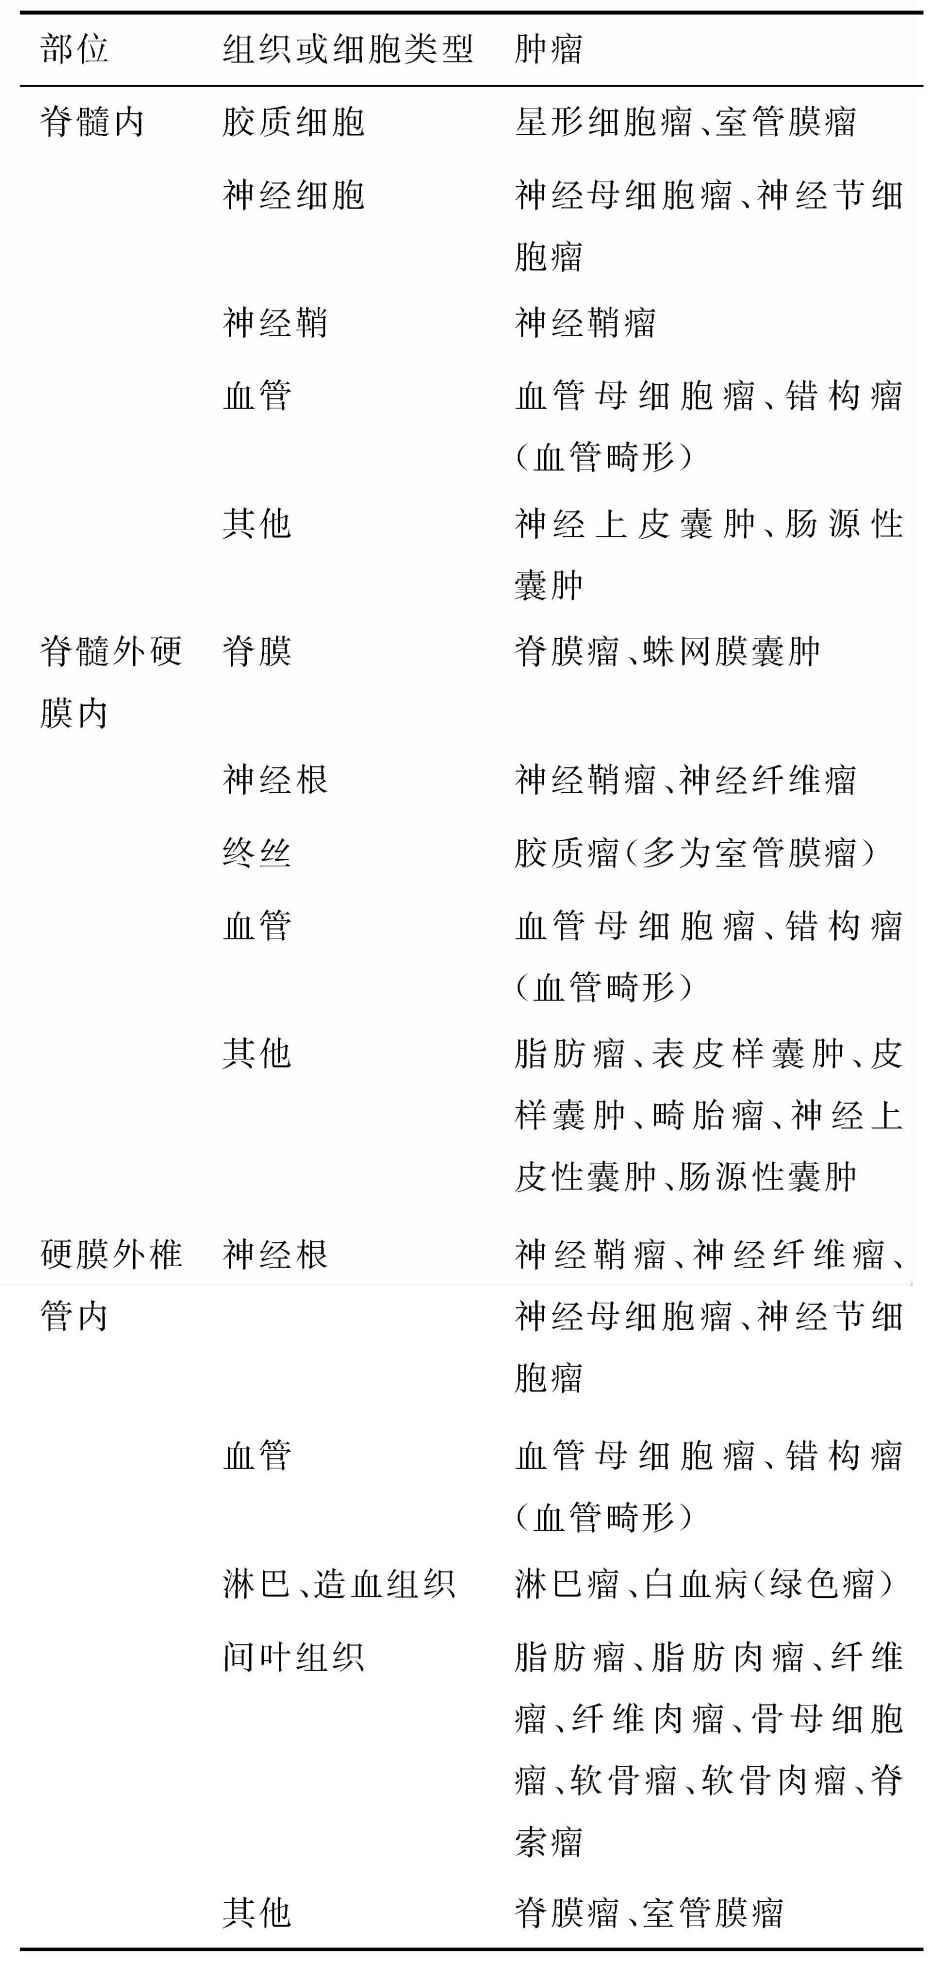
\includegraphics[width=\textwidth,height=\textheight,keepaspectratio]{./images/Image00478.jpg}
\end{table}

1.髓内肿瘤:占椎管内肿瘤的10%~15%。绝大多数为胶质瘤(90%~95%),以室管膜瘤和星形细胞瘤最为多见。其中,室管膜瘤占髓内肿瘤的65%。血管母细胞瘤、少枝胶质细胞瘤、髓母细胞瘤较少见。先天性脂肪瘤或皮样囊肿等良性肿瘤更为少见。髓内转移瘤罕见。

2.髓外硬膜下肿瘤:占椎管内肿瘤的60%。绝大部分为良性肿瘤,以神经鞘瘤、神经纤维瘤和脊膜瘤最常见。此类肿瘤生长缓慢,有完整包膜。

3.髓外硬膜外肿瘤:占椎管内肿瘤的25%。绝大部分为恶性肿瘤,可以是椎骨恶性肿瘤的侵入或远处癌肿转移而来,亦可是淋巴瘤、骨髓瘤或肉瘤等原发肿瘤,脂肪瘤偶可发生。肿瘤大多位于硬膜外腔的后方或侧后方,因此处软组织血管丛丰富,而前方仅为潜在腔隙。

4.哑铃状肿瘤:少数肿瘤可同时长在硬膜内外,骑跨于椎间孔处。椎间孔扩大,硬膜有局部缺损。肿瘤大多呈哑铃状,约占椎管内肿瘤的7%,以神经鞘瘤和神经纤维瘤为多。脊膜瘤等偶呈哑铃状生长。

\subsection{脊髓内室管膜瘤}

本病起源于脊髓中央管的室管膜细胞或终丝等部位的室管膜残余组织,约占髓内肿瘤的65%。可发生于脊髓各节段,以上下两端多见,尤以颈髓多见。其中,黏液乳头型好发于终丝、马尾,占马尾、终丝区原发肿瘤的90%。

\textbf{【病理】}
病变范围多较长,可累及数个节段,呈长圆形或腊肠状膨胀性生长,因有假包膜分界清楚。病程较长,可长得很大。组织学上分为乳头型、细胞型、上皮型和混合型,髓内室管膜型主要为细胞型,终丝部位最常见为黏液乳头型,常合并急性蛛网膜下腔出血。该肿瘤30%可囊变,关于钙化的报道仍不很明确。

\textbf{【临床表现】}
好发于20~50岁,男性略多于女性。主要表现为局限背颈痛,可逐渐出现肿瘤节段以下的运动障碍、感觉异常及膀胱功能异常。

\textbf{【CT表现】}
病变处脊髓不规则膨大,呈等或低密度,但极少高于脊髓密度。病变区边缘模糊不清,囊变部分呈低密度。有时可见蛛网膜下腔出血。增强扫描肿瘤实质部分轻度强化,囊变区不强化。也有报道发生于终丝的富血供肿瘤实质部分呈结节状显著强化。延迟扫描时偶见对比剂进入囊腔。CTM可见蛛网膜下腔变窄、闭塞、移位。

\subsection{脊髓内星形细胞瘤}

本病来源于脊髓的星形细胞,约占髓内肿瘤的30%,其中75%发生于颈、胸段。

\textbf{【病理】}
75%是相对良性的(Ⅰ~Ⅱ级),肿瘤常沿脊髓纵轴呈浸润性或膨胀性生长,常累及多个脊髓节段,病变累及范围较室管膜瘤大,少数可累及脊髓全长。肿瘤界限不清。可继发脊髓空洞,文献报道38%可发生囊变。

\textbf{【临床表现】}
多见于30~50岁,男稍多于女,是儿童最常见的髓内肿瘤。临床表现为感觉功能障碍,局部疼痛,有时反复发作腹痛也是早期症状之一。晚期可引起脊髓功能不全症状和体征。

\textbf{【CT表现】}
脊髓呈梭形或不规则增粗,相邻蛛网膜下腔受压、变窄,甚至完全闭塞。偏良性者可见椎管扩大、局部骨质吸收。肿瘤可呈低、等或高密度,钙化少见。增强扫描呈不均匀性强化,较良性者可不强化;于肿瘤中心或表面可见较低密度囊变,不强化,但有时囊变难以清晰显示。肿瘤上下端可见肿瘤性空洞形成,可呈香肠状低密度,亦无强化。CTM可见蛛网膜下腔变窄、闭塞。

\subsection{血管母细胞瘤}

本病又称为成血管细胞瘤。多认为是起源于血管内皮细胞的富血管良性肿瘤,占髓内肿瘤的1%~5%。75%椎管内血管母细胞瘤发生于髓内,好发于颈胸段,有广泛生长的倾向。

\textbf{【病理】}
肿瘤可单发,通常为多发,肿瘤界限明显,但无包膜,脊髓背侧软脊膜上可见粗大血管匍匐。镜下肿瘤实体或结节内见扩张的毛细血管网或海绵状血管网。肿瘤75%~80%有囊变,囊壁上有大小不等的结节,有时囊壁出现钙化,亦可见瘤内出血。

可伴发延髓空洞症和脊髓空洞症,约1/3合并有Von
Hippel-Lindan病(脑、脊髓或视网膜多发血管瘤、胰和肾囊肿、肾癌),或与脊髓血管畸形并存。

\textbf{【临床表现】}
多表现为局部颈背部疼痛和一侧或双侧上肢感觉减退,位置感和振动感消失(背侧脊髓综合征),但感觉障碍的发生水平与肿瘤所在脊髓节段水平常不一致(常偏高)。

\textbf{【CT表现】}
脊髓局限性增粗,有不规则片状略低密度,瘤巢可呈等或稍高密度,有时可见斑点、条状钙化。更低密度的囊变为本病特征之一。增强扫描肿瘤及囊壁结节明显强化,边缘清楚。于脊髓背侧有时见迂曲的血管影。CTM可显示脊髓表面及蛛网膜下腔的迂曲血管影。总之,本病以范围大、明显强化、明显囊变为特征。

\subsection{神经鞘的肿瘤}

\textbf{【病理】} 神经鞘的肿瘤主要有3种病理类型。

1.神经鞘瘤:为最常见的椎管内肿瘤,占所有椎管内肿瘤的29%,起源于神经鞘的雪旺氏细胞,故又称雪旺氏细胞瘤。可发生于脊髓各节段,而以颈胸段略多。呈圆形或椭圆形,有包膜,易囊性变、出血和黄色细胞瘤变,极少钙化。镜下可见密集规则排列的梭形细胞和疏松的黏液样基质。恶变不如神经纤维瘤常见。

2.神经纤维瘤:起源于神经鞘的神经纤维母细胞,在椎管外与神经鞘瘤发病率相近,后者略多;在椎管内后者明显多于前者(神经纤维瘤仅占二者总数的1%)。神经纤维瘤常见于神经纤维瘤病Ⅰ型患者。肿瘤无包膜,界限不清,囊性变罕见。镜下见瘤内有雪旺氏细胞与纤维母细胞,并可见大片分布于无结构黏液基质的胶原纤维。恶变发生率为2%~12%。

3.神经节瘤:常见部位为颞叶与第三脑室底;椎管内者多发生于脊神经,也可见于脊髓。肿瘤边缘清楚,切面可见明显的漩涡状结构。镜下除见雪旺氏细胞与纤维母细胞外,还可见节细胞。当肿瘤内含有肿瘤性胶质细胞时,称为胶质节瘤。

\textbf{【临床表现】}
椎管内神经鞘瘤和神经纤维瘤好发于20~50岁内,男女发病率相近。神经节瘤好发于儿童及少年。临床症状与椎间盘突出相似,均有疼痛、放射性根痛,也可出现感觉异常及肢体力弱,可有脊髓压迫症状。

\textbf{【CT表现】}
平扫常可见椎管或神经孔扩大,椎弓根骨质破坏。肿瘤呈圆形实质性肿块,常比脊髓密度略低或略高。易跨越硬膜囊,向椎间孔方向生长而呈哑铃状,还可见脊髓受压移位。增强扫描可呈中度均一强化,囊变区无强化。CTM可清晰显示阻塞部位、肿瘤与脊髓的分界以及脊髓移位情况,阻塞部位上、下方的蛛网膜下腔常增宽。

CT无法区别神经鞘瘤和神经纤维瘤,但前者易囊变;而后者早期仅见脊神经增粗,且有多发倾向,有时可恶变。

\textbf{【鉴别诊断】}
①主要应与脊膜瘤相鉴别。后者易出现钙化,向椎间孔侵犯者较少,很少出现哑铃状改变;且后者常见于脊髓后方,与神经鞘瘤多居于脊髓侧方不同。②还应与罕见的肥大性神经病(包括家族性特发性肥大性神经病、进行性肌萎缩等)相鉴别。后者病变神经根远端增粗,呈洋葱状,主要应与多发神经根肿瘤如神经纤维瘤病Ⅰ型相鉴别。

\subsection{脊膜瘤}

本病来源于蛛网膜杯状细胞,占所有椎管内肿瘤的25%,其发病率约占椎管内肿瘤的第二位。80%以上发生于胸段;颈段次之,占17%;腰段极少,占7%。肿瘤常位于脊髓背侧(67%)。

\textbf{【病理】}
93%位于髓外硬膜下,5%跨硬膜呈哑铃状生长,5%位于硬膜外。硬膜外者更具侵袭性,其中约1/2属神经纤维瘤病。肿瘤多较小,一般2~3.5cm。常单发圆形或椭圆形,多发罕见,有完整包膜。一般与硬脊膜粘连较紧,很少附着于蛛网膜,极少浸润到脊髓内。脊髓受压部位远端因血供障碍可出现水肿、软化甚至囊变。组织学上以上皮型最常见,纤维母细胞型和砂粒型次之,其他类型少见。镜下大多有钙化,但大的钙化罕见;年龄越大,钙化率越高。少数可恶变。

\textbf{【临床表现】}
发病年龄13~82岁,峰值年龄50~70岁,平均53岁,女性约占80%。主要表现为神经功能损害,90%有运动神经功能损害,感觉障碍约占60%,约50%可有大小便功能障碍与疼痛。脑脊液蛋白含量高。

\textbf{【CT表现】}
平扫多为椭圆形或圆形实性肿块,偶呈哑铃状生长。多较局限,边缘清晰。密度多高于相应脊髓,其内可见到不规则钙化。邻近骨质可有增生性改变。增强扫描肿瘤呈中度强化。CTM可见肿瘤部蛛网膜下腔部分或完全阻塞,脊髓受压变细并有明显移位。

\subsection{硬膜外转移瘤}

硬膜外转移瘤的部位和发病率常与椎体转移瘤密切相关,两者常同时存在,有时难以区分起源于硬膜外还是椎体。

\textbf{【病因】}
其转移途径有:①经动脉播散;②经椎静脉播散;③经淋巴系统播散;④经蛛网膜下腔播散;⑤邻近病灶直接侵入椎管。

肿瘤常见原发灶为:①血行转移主要来自肺癌、乳癌、肾癌、甲状腺癌和前列腺癌等,可影响椎体和附件。②恶性淋巴瘤可经淋巴系统侵犯椎管内结构,亦常分布于硬膜外,但较少累及椎体。③颅内髓母细胞瘤、室管膜瘤可通过脑脊液循环种植而来,常易侵犯硬脊膜,可单发或多发。④白血病及黑色素瘤可以浸润至硬脊膜、脊髓或神经根,如白血病呈结节状增殖易产生严重的脊髓受压。

\textbf{【临床表现】}
早期无明显症状,后期可出现单肢瘫痪、根性疼痛、感觉异常和步态异常等马尾神经损害表现。

\textbf{【CT表现】}
主要为硬膜外可见到不规则软组织肿块,易向椎旁软组织内侵犯,硬膜囊和脊髓有不同程度的受压、移位。有些肿瘤可穿破硬脊膜向硬膜下或髓内生长,而致脊髓外形不规则。增强扫描部分肿瘤可强化。常伴有邻近椎骨破坏,特别是椎弓根溶骨性破坏,椎间隙多无狭窄。此外,应注意结合原发肿瘤病史诊断。

\textbf{【鉴别诊断】}
有时需与慢性肉芽肿性炎症相鉴别。后者常有感染病史;邻近骨质破坏的边缘常有硬化带出现,有时可见骨质增生;病变向周围浸润较少见;增强扫描常无明显强化。

\subsection{椎管内淋巴瘤}

淋巴瘤常累及椎管,较颅内多2~3倍,以硬膜外或硬膜受侵最多见。

\textbf{【病理】}
也分为霍奇金病和非霍奇金林巴瘤。肿瘤最易通过椎间孔直接侵犯到椎旁或硬膜外腔,常围绕硬膜囊及神经根生长,硬膜囊呈多节段的环状狭窄。有时肿瘤可经血管周围间隙侵犯脊髓实质,偶可使周围静脉和毛细血管破裂而致硬膜下血肿,椎体骨质亦可受累。本病常累及胸腰椎。

\textbf{【临床表现】}
多见于男性,发病年龄不甚一致。临床主要表现为脊髓和神经根受压症状,以局部神经痛最常见,逐渐出现下肢运动、感觉障碍和括约肌功能紊乱。

\textbf{【CT表现】}
原发性者其特征性表现为病灶起自脊髓的后侧或后外侧,呈浸润性生长,肿瘤包绕脊髓背侧并挤压脊髓,邻近椎体、椎旁软组织往往受累。继发性者可见到以软组织密度为主的椎旁肿块并从椎间孔侵入硬膜外腔,或以溶骨性的脊椎破坏为主要表现。肿瘤多呈实质性,密度均匀。硬膜囊变窄甚至闭塞;脊髓受压、移位,常累及多个脊髓节段。增强扫描呈不规则强化。

本病应注意与椎旁肌肉或结缔组织的原发肿瘤及某些感染性疾病相鉴别,必要时穿刺活检。

\subsection{表皮样囊肿}

本病罕见,占脊髓肿瘤的0.5%~1%。

\textbf{【病因病理】}
根据其来源可分为两类:①先天性:来自皮肤外胚层,常伴有相关骨结构异常如脊柱裂、半椎畸形等,20%合并背侧皮窦。②获得性:约占40%,为腰椎穿刺的晚期合并症,发病时距腰穿1~20年。来自穿刺时植入硬膜囊内的皮肤生发层细胞,常与神经根及软脊膜粘连,不伴脊柱骨结构的异常。

囊肿壁薄而透明,内容物为角化物、胆固醇结晶、蛋白质等,其内不含毛发、皮脂腺,囊壁为鳞状上皮,通常无钙化。

\textbf{【临床表现】}
多见于儿童,为儿童椎管内肿瘤的10%;也可见于成人,好发年龄为20~30岁,男性多见,男女之比为8∶1。临床主要表现为进行性腰背痛及下肢放射性痛等,可出现脊柱前突及步态异常。

\textbf{【CT表现】}
平扫或CTM可见腰或下胸段髓外硬膜下较低的软组织密度,马尾神经推向一侧。大者可造成硬膜囊梗阻。发生于圆锥的囊肿,与圆锥不能区分。增强扫描病灶无强化。先天性可见相关脊柱异常。

本病与其他髓外硬膜下占位不易鉴别。

\subsection{皮样囊肿}

本病罕见,为胚胎残余组织的良性肿瘤。

\textbf{【病理】}
病灶位于髓外硬膜下,罕见于髓内,常见于腰段。来自胚胎时期原始神经管形成过程中,皮肤外胚层包涵于神经管内。与表皮样囊肿不同的是其内常见皮肤的各种成分,呈干酪样物质。内容物为角化物、毛发和液态胆固醇,囊壁为皮肤组织、鳞状上皮、皮肤附属器、皮脂腺,常见钙化。囊肿可破裂而引起化学性蛛网膜炎,有恶变为鳞癌的报道。

\textbf{【临床表现】}
多见于婴儿,占1岁以内硬膜下肿瘤的20%,但由于生长缓慢,多于成人出现症状。也主要表现为进行性腰背痛及下肢放射性痛等。

\textbf{【CT表现】}
大多位于腰骶部,多合并隐性脊柱裂。平扫囊肿呈硬膜囊内占位,密度常接近脂肪密度;CT不易显示囊肿破裂后的脂肪类内容物在硬膜囊内的播散与蛛网膜炎的增强表现。如病灶内显示钙化则提示畸胎瘤。

\subsection{蛛网膜囊肿}

根据其发病部位及是否与蛛网膜下腔相通分别被称为蛛网膜囊肿、脊膜囊肿、蛛网膜憩室、硬膜外囊肿及神经周围囊肿或神经根袖扩张。

\textbf{【病因病理】}
其病因尚未完全肯定,可分为原发性和继发性。一般认为与先天性蛛网膜和(或)硬脊膜发育不良有关,而非肿瘤性病变;也可能与外伤、出血、炎症等有关。根据病变部位将其分为与硬膜囊有关及神经根有关两大组,前者又分为硬膜下和硬膜外两类。多数囊肿与蛛网膜下腔相通。囊肿含有脑脊液,包膜主要由硬膜囊、神经根鞘膜或蛛网膜组成。

\textbf{【临床表现】}
本病男性略多见,出现症状平均年龄约50岁。主要为不同程度的脊髓或神经根感觉与运动异常,如颈部、腰背部或四肢疼痛、肢体乏力、大小便功能障碍等。

\textbf{【CT表现】}
①椎管内大小、长短不一的水样密度灶,有时可沿椎间孔向椎管外生长,并可沿脊神经分叉而分叉,增强扫描无强化。②大多数椎管及椎间孔有不同程度的扩大,表现为以病变为中心向四周(向外)膨隆的弧形压迹,边缘光滑、清晰锐利。③CTM有时可见囊肿充盈造影剂,亦可不能显示囊肿,而表现为脊髓神经根受压移位。④一般CT平扫和增强扫描难以确定与硬脊膜或脊髓的关系,亦常不能确定囊肿是否有孔或蒂与蛛网膜下腔相通。

\textbf{【鉴别诊断】}
本病需注意与表皮样囊肿、皮样囊肿、畸胎瘤、肠源性囊肿等相鉴别,但CT鉴别可能困难。

\protect\hypertarget{text00031.html}{}{}

